\chapter{Differentially heated cavity}

The differentially heated cavity problem or buoyancy-driven cavity problem is a two dimensional problem based on free convection. It comprises a cavity with the vertical walls at different temperatures and adiabatic horizontal walls \cite{DeVahlDavis1983a, DeVahlDavis1983}. The difference of temperatures between the two vertical walls causes convection.

\begin{figure}[h]
	\centering
	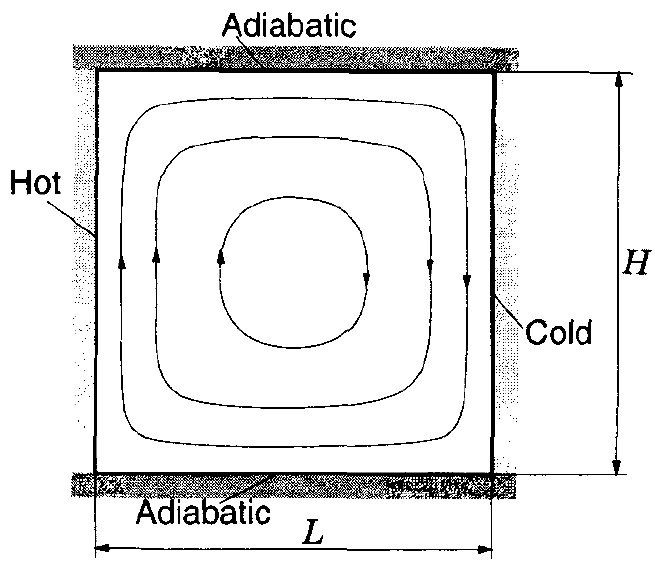
\includegraphics[scale=0.5]{Buoyancy/BuoyancyDriven}
	\caption[General scheme of the differentially heated problem]{General scheme of the differentially heated problem. Extracted from \cite{Ferziger2002}}
\end{figure}

\section{Natural convection}
The equations that are going to be discretized are the two-dimensional equations of mass, momentum and energy for a Newtonian fluid with constant properties. However, some approximations have to be done for the momentum equation:
\begin{equation}
\rho_{0}\frac{\partial\vec{v}}{\partial t}+\rho_{0}\left(\vec{v}\cdot\nabla\right)\vec{v}=-\nabla p+\mu\nabla^{2}\vec{v}+\rho\vec{g}
\end{equation}
As it can be seen, mass forces have been added to the momentum equation, because in natural convection gravity is not negligible. Another important remark is that the fluid is considered incompressible, but this approximation is not applied in the gravitational term, because it is this term that causes the flow. However, as a simplification, the Boussinesq approximation is applied \cite{Bergman2011,Ghiaasiaan2011}:
\begin{equation}
\rho=\rho_{0}\left(1-\beta\left(T-T_{0}\right)\right)
\end{equation}
where $\beta$ is the volumetric thermal expansion coefficient, a thermodynamic property that measures the variation of the density as a function of the temperature at a constant pressure.
Introducing the Boussinesq approximation in the momentum equation, the final equations for natural convection are:
\begin{equation}
\nabla\cdot\vec{v}=0
\label{NatConvContinuity}
\end{equation}
\begin{equation}
\rho_{0}\frac{\partial\vec{v}}{\partial t}+\rho_{0}\left(\vec{v}\cdot\nabla\right)\vec{v}=-\nabla p_{d}+\mu\nabla^{2}\vec{v}-\rho_{0}\beta\left(T-T_{0}\right)\vec{g}
\label{NatConvMomentum}
\end{equation}
\begin{equation}
\rho c_{p}\left(\frac{\partial T}{\partial t}+\vec{v}\cdot\nabla T\right)=\lambda\nabla^{2}T
\label{NatConvEnergy}
\end{equation}

\subsection{Non-dimensional equations}
In order to have a simpler analysis, it is convenient to use non-dimensional variables. Depending on the problem, they can be defined by several different ways. In this section, taking into account the most important variables of a free convection problem, the dimensionless variables are defined as it is expressed below:
\begin{equation}
\vec{x}^{*}=\frac{\vec{x}}{L}
\end{equation}
\begin{equation}
\vec{v}^{*}=\frac{\vec{v}}{\frac{\lambda}{\rho Lc_{P}}}
\end{equation}
\begin{equation}
t^{*}=\frac{t}{\frac{\rho L^{2}c_{P}}{\lambda}}
\end{equation}
\begin{equation}
p^{*}=\frac{p}{\frac{1}{\rho}\left(\frac{\lambda}{c_{P}L}\right)^2}
\end{equation}
\begin{equation}
T^{*}=\frac{T-T_{cold}}{T_{hot}-T_{cold}}
\label{DimensionlessTemperature}
\end{equation}
Inserting these expressions in the equations \ref{NatConvContinuity}, \ref{NatConvMomentum} and \ref{NatConvEnergy}, the non-dimensional equations for natural convection are obtained. In order to simplify the notation, the indexes $^{*}$ have been removed, but the variables that are represented in the following section are the dimensionless ones.
\begin{equation}
\nabla\cdot\vec{v}=0
\end{equation}
\begin{equation}
\frac{\partial\vec{v}}{\partial t}+\left(\vec{v}\cdot\nabla\right)\vec{v}=-\nabla p+Pr\nabla^{2}\vec{v}-PrRaT\vec{u}_{g}
\end{equation}
\begin{equation}
\frac{\partial T}{\partial t}+\vec{v}\cdot\nabla T=\nabla^{2}T
\end{equation}

The dimensionless numbers that appear are the Prandtl and Rayleigh numbers, defined as:
\begin{equation}
Pr\equiv\frac{c_{P}\mu}{\lambda}
\end{equation}
\begin{equation}
Ra\equiv\frac{\rho^{2} g\beta\Delta TL^{3}c_{P}}{\mu\lambda}
\end{equation}
where $\Delta T=T_{hot}-T_{cold}$.

\section{Application of the fractional step method}
The resolution of this problem can be done using the fractional step method described in chapter \ref{FractionalStepM}. In the case of the momentum equation its resolution is done as it is explained in the mentioned section. But the expression of the equation is slightly different. Rewritting the momentum equation as it was done:
\begin{equation}
\frac{\partial\vec{v}}{\partial t}=R\left(\vec{v}\right)-\nabla p
\end{equation}
where
\begin{equation}
R\left(\vec{v}\right)=-\left(\vec{v}\cdot\nabla\right)\vec{v}+Pr\nabla^{2}\vec{v}-PrRaT\vec{u}_{g}
\end{equation}

The other important issue is the introduction of the energy equation. It has to be discretized according to the fractional step method. As it can be seen, this case is very similar to the previously studied Smith-Hutton problem, since the velocity field is "known" (calculated by other means) and the unknown is a scalar. Therefore, an implicit scheme is going to be used for the temporal integration:
\begin{equation}
\frac{T^{n+1}-T^{n}}{\Delta t}=\left[-\vec{v}\cdot\nabla T+\nabla^{2}T\right]^{n+1}
\end{equation}

\section{Discretization}
The spatial discretization of the domain is the one described by the figure \ref{staggered}: a Cartesian grid with a staggered mesh.

The discretization of the momentum equation is very similar to that described in the fractional step method chapter but adding the gravity term in the case of the vertical equation:
\begin{multline}
	R\left(u\right)V_{P}=\left[Pr_{e}\frac{u_{E}-u_{P}}{d_{EP}}A_{e}+Pr_{n}\frac{u_{N}-u_{P}}{d_{NP}}A_{n}-Pr_{w}\frac{u_{P}-u_{W}}{d_{WP}}A_{w}-Pr_{s}\frac{u_{P}-u_{S}}{d_{SP}}A_{s}\right] \\
	-\left[\left(u\right)_{e}u_{e}A_{e}+\left(v\right)_{n}u_{n}A_{n}-\left(u\right)_{w}u_{w}A_{w}-\left(v\right)_{s}u_{s}A_{s}\right]
\end{multline}
\begin{multline}
	R\left(v\right)V_{P}=\left[Pr_{e}\frac{v_{E}-v_{P}}{d_{EP}}A_{e}+Pr_{n}\frac{v_{N}-v_{P}}{d_{NP}}A_{n}-Pr_{w}\frac{v_{P}-v_{W}}{d_{WP}}A_{w}-Pr_{s}\frac{v_{P}-v_{S}}{d_{SP}}A_{s}\right] \\
	-\left[\left(u\right)_{e}v_{e}A_{e}+\left(v\right)_{n}v_{n}A_{n}-\left(u\right)_{w}v_{w}A_{w}-\left(v\right)_{s}v_{s}A_{s}\right]+PrRaTV_{P}
\end{multline}

In the case of the energy equation a similar approach is used. Temperature, like pressure, is evaluated in the nodes, not in the faces like the velocities. The integration of the terms of the equations starts with the Gauss Theorem:
\begin{equation}
\int_{\Omega}\vec{v}\nabla Td\Omega=\int_{\partial\Omega}\vec{v}\cdot\vec{n} TdS\approx\left(u\right)_{e}T_{e}A_{e}+\left(v\right)_{n}T_{n}A_{n}-\left(u\right)_{w}T_{w}A_{w}-\left(v\right)_{s}T_{s}A_{s}
\end{equation}
\begin{equation}
	\int_{\Omega}\nabla^{2}Td\Omega=\int_{\partial\Omega}\nabla TdS\approx\frac{T_{E}-T_{P}}{d_{PE}}A_{e}+\frac{T_{N}-T_{P}}{d_{PN}}A_{n}-\frac{T_{P}-T_{W}}{d_{PW}}A_{w}-\frac{T_{P}-T_{S}}{d_{PS}}A_{s}
\end{equation}
The temperature in the faces is evaluated using the central differencing scheme, as it was done for the velocities.

The final discretized equation for the temperature can be expressed as:
\begin{equation}
a_{P}T_{P}=a_{E}T_{E}+a_{W}T_{W}+a_{N}T_{N}+a_{S}T_{S}+b_{p}
\end{equation}
where the discretized coefficients are the same discussed in section \ref{FinalDiscretizationGCDE} for a central differencing scheme.

\section{Boundary conditions}
Since the cavity is all surrounded by walls, the boundary velocities are:
\begin{itemize}
	\item $\vec{v}=0$ in the top wall
	\item $\vec{v}=0$ in the bottom wall
	\item $\vec{v}=0$ in the left wall
	\item $\vec{v}=0$ in the right wall
\end{itemize}
In the case of the temperature, they are determined in the right and left walls. Taking into account the expression of T in the equation \ref{DimensionlessTemperature}:
\begin{itemize}
	\item $T=1$ in the left wall
	\item $T=0$ in the right wall
\end{itemize}
In the top and bottom walls the only condition is that they are adiabatic. This condition can also be expressed as:
\begin{equation}
\frac{\partial T}{\partial y}\approx\frac{T_{P}-T_{S}}{d_{PS}}=0
\end{equation}
\begin{equation}
T_{P}=T_{S}
\end{equation}
As a consequence, the discretized coefficients of the boundary nodes have the values listed in table \ref{BoundTempDiffHeat}.
\begin{table}[h]
	\centering\begin{tabular}{ |c|c|c|c|c| }
		\hline
		Coefficients & Left & Right & Top & Bottom \\ \hline
		$a_{E}$ & $0$ & $0$ & $0$ & $0$ \\ \hline
		$a_{W}$ & $0$ & $0$ & $0$ & $0$ \\ \hline
		$a_{N}$ & $0$ & $0$ & $0$ & $1$ \\ \hline
		$a_{S}$ & $0$ & $0$ & $1$ & $0$ \\ \hline
		$a_{P}$ & $1$ & $1$ & $1$ & $1$ \\ \hline
		$b_{P}$ & $0$ & $1$ & $0$ & $0$ \\ \hline
	\end{tabular}
\caption{Discretization coefficients of the boundary temperature nodes}
\label{BoundTempDiffHeat}
\end{table}

\section{Nusselt number}
In the differentially heated cavity, the motion occurs due to the convective transfer. In other words, the temperature gradient is the important issue in this problem, so it would be useful to calculate it. The local heat flux in a horizontal direction at any point in the cavity \cite{DeVahlDavis1983}:
\begin{equation}
Q\left(x, y\right)=uT-\frac{\partial T}{\partial x}
\end{equation}
The Nusselt number is a non-dimensional parameter that can be seen as the dimensionless temperature gradient. It provides a measure of the convection heat at a surface \cite{Bergman2011}. The local Nusselt number gives the heat flow through any vertical line:
\begin{equation}
	Nu_{x}=\int_{0}^{1}Q\left(x, y\right)dy
\end{equation}
Another useful value is the average Nusselt number of the whole cavity:
\begin{equation}
\overbar{Nu}=\int_{0}^{1}Nu_{x}dx
\end{equation}

\section{Algorithm}
The algorithm used to calculate this problem is very similar to that of the driven cavity problem, but adding the resolution of the temperature. As in the previous program, the simulation ends when the cavity reaches a steady state.
\begin{figure}[H]
	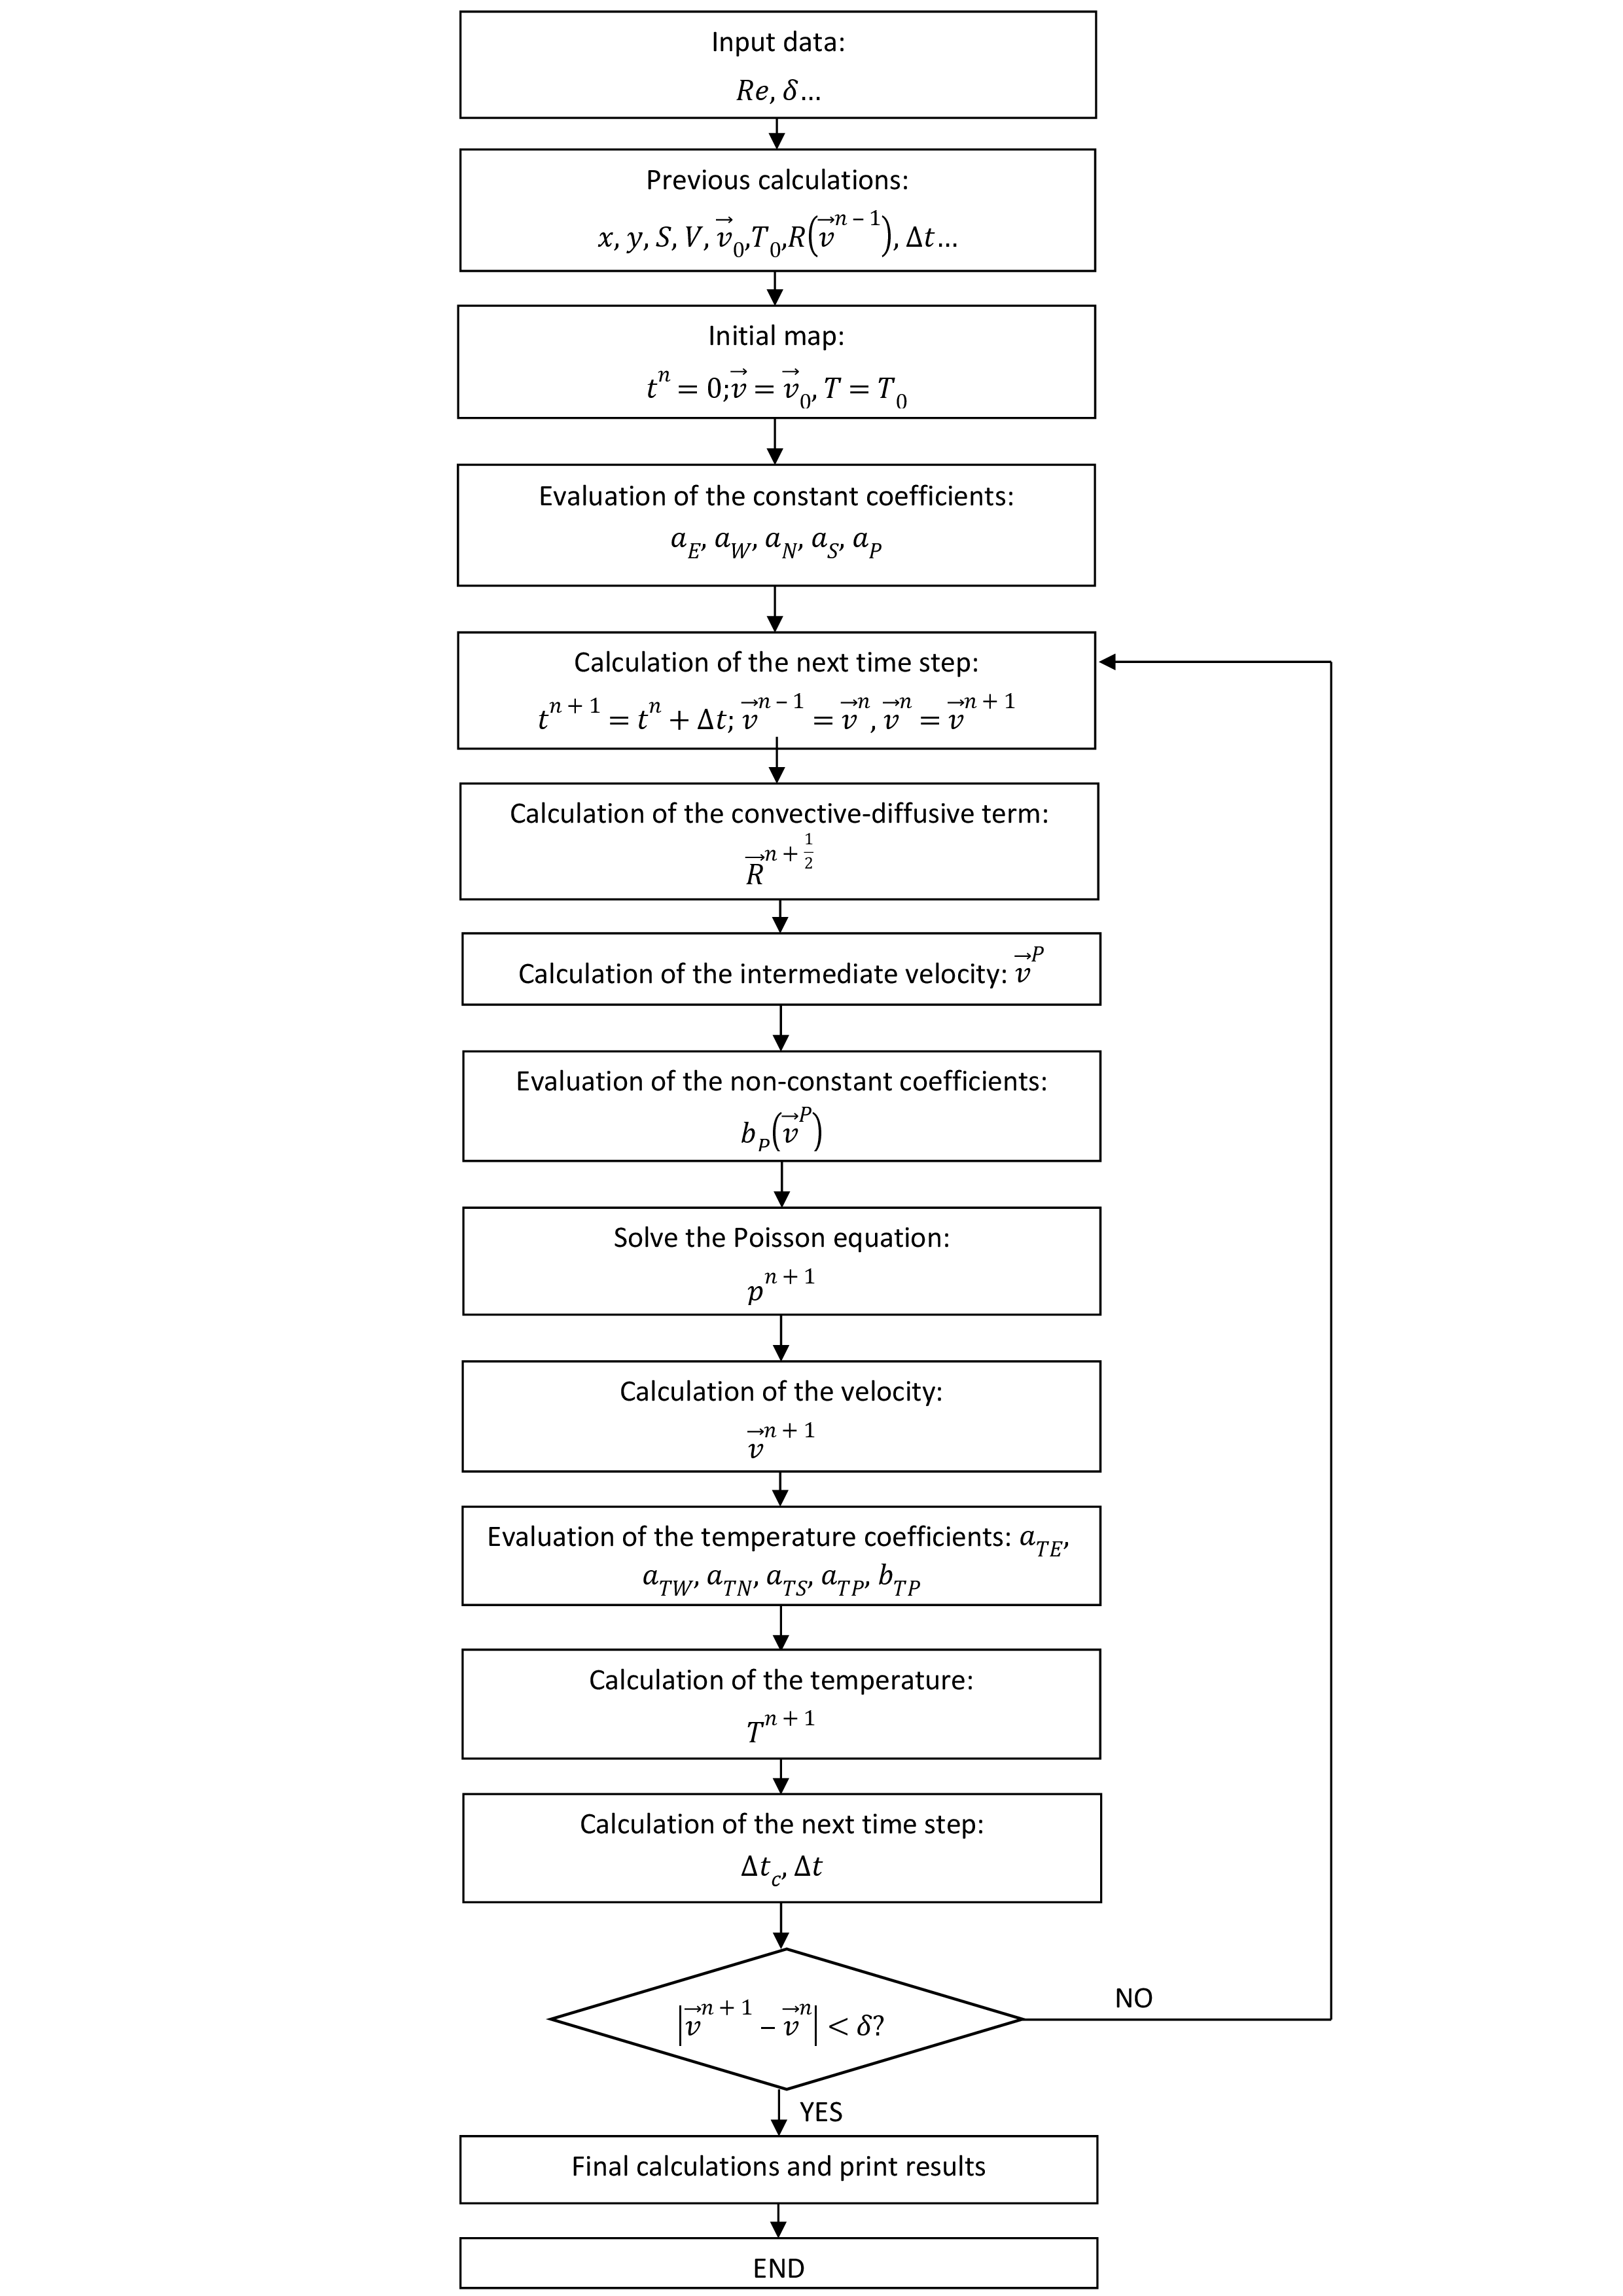
\includegraphics[scale=0.185]{Buoyancy/Doc4}
\end{figure}

\section{Results}
In order to provide different ranges of solutions, the code has been tested for different Rayleigh numbers. The parameters of the simulations are listed in table \ref{NumericalParamDiffHeated}.
\begin{table}[H]
	\centering
	\begin{tabular}{ |c|c|c|c|c| }
		\hline
		$N$ & $M$ & $L$ & $Pr$ & $\delta$ \\ \hline
		$50$ & $50$ & $1$ & $0.71$ & $10^{-4}$ \\ \hline
	\end{tabular}
\caption{Numerical parameters of the differentially heated cavity problem}
\label{NumericalParamDiffHeated}
\end{table}
\begin{figure}[h]
	\begin{subfigure}{0.5\textwidth}
		\resizebox{1.4\textwidth}{!}{% GNUPLOT: LaTeX picture with Postscript
\begingroup
  \makeatletter
  \providecommand\color[2][]{%
    \GenericError{(gnuplot) \space\space\space\@spaces}{%
      Package color not loaded in conjunction with
      terminal option `colourtext'%
    }{See the gnuplot documentation for explanation.%
    }{Either use 'blacktext' in gnuplot or load the package
      color.sty in LaTeX.}%
    \renewcommand\color[2][]{}%
  }%
  \providecommand\includegraphics[2][]{%
    \GenericError{(gnuplot) \space\space\space\@spaces}{%
      Package graphicx or graphics not loaded%
    }{See the gnuplot documentation for explanation.%
    }{The gnuplot epslatex terminal needs graphicx.sty or graphics.sty.}%
    \renewcommand\includegraphics[2][]{}%
  }%
  \providecommand\rotatebox[2]{#2}%
  \@ifundefined{ifGPcolor}{%
    \newif\ifGPcolor
    \GPcolortrue
  }{}%
  \@ifundefined{ifGPblacktext}{%
    \newif\ifGPblacktext
    \GPblacktexttrue
  }{}%
  % define a \g@addto@macro without @ in the name:
  \let\gplgaddtomacro\g@addto@macro
  % define empty templates for all commands taking text:
  \gdef\gplbacktext{}%
  \gdef\gplfronttext{}%
  \makeatother
  \ifGPblacktext
    % no textcolor at all
    \def\colorrgb#1{}%
    \def\colorgray#1{}%
  \else
    % gray or color?
    \ifGPcolor
      \def\colorrgb#1{\color[rgb]{#1}}%
      \def\colorgray#1{\color[gray]{#1}}%
      \expandafter\def\csname LTw\endcsname{\color{white}}%
      \expandafter\def\csname LTb\endcsname{\color{black}}%
      \expandafter\def\csname LTa\endcsname{\color{black}}%
      \expandafter\def\csname LT0\endcsname{\color[rgb]{1,0,0}}%
      \expandafter\def\csname LT1\endcsname{\color[rgb]{0,1,0}}%
      \expandafter\def\csname LT2\endcsname{\color[rgb]{0,0,1}}%
      \expandafter\def\csname LT3\endcsname{\color[rgb]{1,0,1}}%
      \expandafter\def\csname LT4\endcsname{\color[rgb]{0,1,1}}%
      \expandafter\def\csname LT5\endcsname{\color[rgb]{1,1,0}}%
      \expandafter\def\csname LT6\endcsname{\color[rgb]{0,0,0}}%
      \expandafter\def\csname LT7\endcsname{\color[rgb]{1,0.3,0}}%
      \expandafter\def\csname LT8\endcsname{\color[rgb]{0.5,0.5,0.5}}%
    \else
      % gray
      \def\colorrgb#1{\color{black}}%
      \def\colorgray#1{\color[gray]{#1}}%
      \expandafter\def\csname LTw\endcsname{\color{white}}%
      \expandafter\def\csname LTb\endcsname{\color{black}}%
      \expandafter\def\csname LTa\endcsname{\color{black}}%
      \expandafter\def\csname LT0\endcsname{\color{black}}%
      \expandafter\def\csname LT1\endcsname{\color{black}}%
      \expandafter\def\csname LT2\endcsname{\color{black}}%
      \expandafter\def\csname LT3\endcsname{\color{black}}%
      \expandafter\def\csname LT4\endcsname{\color{black}}%
      \expandafter\def\csname LT5\endcsname{\color{black}}%
      \expandafter\def\csname LT6\endcsname{\color{black}}%
      \expandafter\def\csname LT7\endcsname{\color{black}}%
      \expandafter\def\csname LT8\endcsname{\color{black}}%
    \fi
  \fi
    \setlength{\unitlength}{0.0500bp}%
    \ifx\gptboxheight\undefined%
      \newlength{\gptboxheight}%
      \newlength{\gptboxwidth}%
      \newsavebox{\gptboxtext}%
    \fi%
    \setlength{\fboxrule}{0.5pt}%
    \setlength{\fboxsep}{1pt}%
\begin{picture}(7200.00,5040.00)%
    \gplgaddtomacro\gplbacktext{%
    }%
    \gplgaddtomacro\gplfronttext{%
      \put(1908,624){\makebox(0,0){\strut{}$0$}}%
      \put(2585,624){\makebox(0,0){\strut{}$0.2$}}%
      \put(3262,624){\makebox(0,0){\strut{}$0.4$}}%
      \put(3938,624){\makebox(0,0){\strut{}$0.6$}}%
      \put(4615,624){\makebox(0,0){\strut{}$0.8$}}%
      \put(5292,624){\makebox(0,0){\strut{}$1$}}%
      \put(1720,938){\makebox(0,0)[r]{\strut{}$0$}}%
      \put(1720,1615){\makebox(0,0)[r]{\strut{}$0.2$}}%
      \put(1720,2292){\makebox(0,0)[r]{\strut{}$0.4$}}%
      \put(1720,2968){\makebox(0,0)[r]{\strut{}$0.6$}}%
      \put(1720,3645){\makebox(0,0)[r]{\strut{}$0.8$}}%
      \put(1720,4322){\makebox(0,0)[r]{\strut{}$1$}}%
      \put(5678,938){\makebox(0,0)[l]{\strut{}$0$}}%
      \put(5678,1614){\makebox(0,0)[l]{\strut{}$0.2$}}%
      \put(5678,2291){\makebox(0,0)[l]{\strut{}$0.4$}}%
      \put(5678,2968){\makebox(0,0)[l]{\strut{}$0.6$}}%
      \put(5678,3645){\makebox(0,0)[l]{\strut{}$0.8$}}%
      \put(5678,4322){\makebox(0,0)[l]{\strut{}$1$}}%
    }%
    \gplbacktext
    \put(0,0){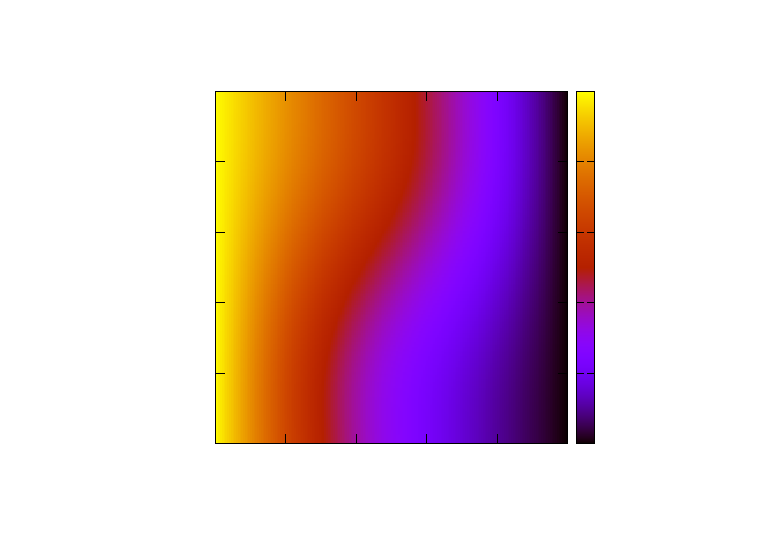
\includegraphics{Buoyancy/T3}}%
    \gplfronttext
  \end{picture}%
\endgroup
}
		\caption{$Ra=10^{3}$}
	\end{subfigure}%
	\begin{subfigure}{0.5\textwidth}
		\resizebox{1.4\textwidth}{!}{% GNUPLOT: LaTeX picture with Postscript
\begingroup
  \makeatletter
  \providecommand\color[2][]{%
    \GenericError{(gnuplot) \space\space\space\@spaces}{%
      Package color not loaded in conjunction with
      terminal option `colourtext'%
    }{See the gnuplot documentation for explanation.%
    }{Either use 'blacktext' in gnuplot or load the package
      color.sty in LaTeX.}%
    \renewcommand\color[2][]{}%
  }%
  \providecommand\includegraphics[2][]{%
    \GenericError{(gnuplot) \space\space\space\@spaces}{%
      Package graphicx or graphics not loaded%
    }{See the gnuplot documentation for explanation.%
    }{The gnuplot epslatex terminal needs graphicx.sty or graphics.sty.}%
    \renewcommand\includegraphics[2][]{}%
  }%
  \providecommand\rotatebox[2]{#2}%
  \@ifundefined{ifGPcolor}{%
    \newif\ifGPcolor
    \GPcolortrue
  }{}%
  \@ifundefined{ifGPblacktext}{%
    \newif\ifGPblacktext
    \GPblacktexttrue
  }{}%
  % define a \g@addto@macro without @ in the name:
  \let\gplgaddtomacro\g@addto@macro
  % define empty templates for all commands taking text:
  \gdef\gplbacktext{}%
  \gdef\gplfronttext{}%
  \makeatother
  \ifGPblacktext
    % no textcolor at all
    \def\colorrgb#1{}%
    \def\colorgray#1{}%
  \else
    % gray or color?
    \ifGPcolor
      \def\colorrgb#1{\color[rgb]{#1}}%
      \def\colorgray#1{\color[gray]{#1}}%
      \expandafter\def\csname LTw\endcsname{\color{white}}%
      \expandafter\def\csname LTb\endcsname{\color{black}}%
      \expandafter\def\csname LTa\endcsname{\color{black}}%
      \expandafter\def\csname LT0\endcsname{\color[rgb]{1,0,0}}%
      \expandafter\def\csname LT1\endcsname{\color[rgb]{0,1,0}}%
      \expandafter\def\csname LT2\endcsname{\color[rgb]{0,0,1}}%
      \expandafter\def\csname LT3\endcsname{\color[rgb]{1,0,1}}%
      \expandafter\def\csname LT4\endcsname{\color[rgb]{0,1,1}}%
      \expandafter\def\csname LT5\endcsname{\color[rgb]{1,1,0}}%
      \expandafter\def\csname LT6\endcsname{\color[rgb]{0,0,0}}%
      \expandafter\def\csname LT7\endcsname{\color[rgb]{1,0.3,0}}%
      \expandafter\def\csname LT8\endcsname{\color[rgb]{0.5,0.5,0.5}}%
    \else
      % gray
      \def\colorrgb#1{\color{black}}%
      \def\colorgray#1{\color[gray]{#1}}%
      \expandafter\def\csname LTw\endcsname{\color{white}}%
      \expandafter\def\csname LTb\endcsname{\color{black}}%
      \expandafter\def\csname LTa\endcsname{\color{black}}%
      \expandafter\def\csname LT0\endcsname{\color{black}}%
      \expandafter\def\csname LT1\endcsname{\color{black}}%
      \expandafter\def\csname LT2\endcsname{\color{black}}%
      \expandafter\def\csname LT3\endcsname{\color{black}}%
      \expandafter\def\csname LT4\endcsname{\color{black}}%
      \expandafter\def\csname LT5\endcsname{\color{black}}%
      \expandafter\def\csname LT6\endcsname{\color{black}}%
      \expandafter\def\csname LT7\endcsname{\color{black}}%
      \expandafter\def\csname LT8\endcsname{\color{black}}%
    \fi
  \fi
    \setlength{\unitlength}{0.0500bp}%
    \ifx\gptboxheight\undefined%
      \newlength{\gptboxheight}%
      \newlength{\gptboxwidth}%
      \newsavebox{\gptboxtext}%
    \fi%
    \setlength{\fboxrule}{0.5pt}%
    \setlength{\fboxsep}{1pt}%
\begin{picture}(7200.00,5040.00)%
    \gplgaddtomacro\gplbacktext{%
    }%
    \gplgaddtomacro\gplfronttext{%
      \put(1908,624){\makebox(0,0){\strut{}$0$}}%
      \put(2585,624){\makebox(0,0){\strut{}$0.2$}}%
      \put(3262,624){\makebox(0,0){\strut{}$0.4$}}%
      \put(3938,624){\makebox(0,0){\strut{}$0.6$}}%
      \put(4615,624){\makebox(0,0){\strut{}$0.8$}}%
      \put(5292,624){\makebox(0,0){\strut{}$1$}}%
      \put(1720,938){\makebox(0,0)[r]{\strut{}$0$}}%
      \put(1720,1615){\makebox(0,0)[r]{\strut{}$0.2$}}%
      \put(1720,2292){\makebox(0,0)[r]{\strut{}$0.4$}}%
      \put(1720,2968){\makebox(0,0)[r]{\strut{}$0.6$}}%
      \put(1720,3645){\makebox(0,0)[r]{\strut{}$0.8$}}%
      \put(1720,4322){\makebox(0,0)[r]{\strut{}$1$}}%
      \put(5678,938){\makebox(0,0)[l]{\strut{}$0$}}%
      \put(5678,1614){\makebox(0,0)[l]{\strut{}$0.2$}}%
      \put(5678,2291){\makebox(0,0)[l]{\strut{}$0.4$}}%
      \put(5678,2968){\makebox(0,0)[l]{\strut{}$0.6$}}%
      \put(5678,3645){\makebox(0,0)[l]{\strut{}$0.8$}}%
      \put(5678,4322){\makebox(0,0)[l]{\strut{}$1$}}%
    }%
    \gplbacktext
    \put(0,0){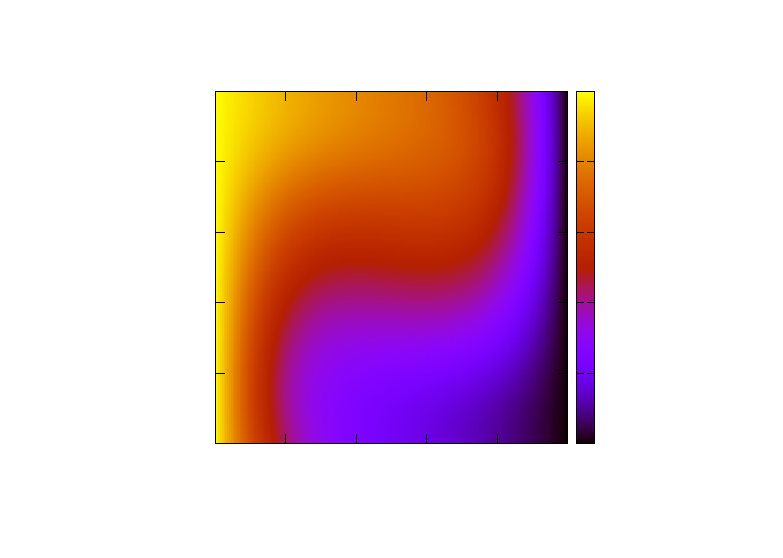
\includegraphics{Buoyancy/T4}}%
    \gplfronttext
  \end{picture}%
\endgroup
}
		\caption{$Ra=10^{4}$}
	\end{subfigure}
	\begin{subfigure}{0.5\textwidth}
		\resizebox{1.4\textwidth}{!}{% GNUPLOT: LaTeX picture with Postscript
\begingroup
  \makeatletter
  \providecommand\color[2][]{%
    \GenericError{(gnuplot) \space\space\space\@spaces}{%
      Package color not loaded in conjunction with
      terminal option `colourtext'%
    }{See the gnuplot documentation for explanation.%
    }{Either use 'blacktext' in gnuplot or load the package
      color.sty in LaTeX.}%
    \renewcommand\color[2][]{}%
  }%
  \providecommand\includegraphics[2][]{%
    \GenericError{(gnuplot) \space\space\space\@spaces}{%
      Package graphicx or graphics not loaded%
    }{See the gnuplot documentation for explanation.%
    }{The gnuplot epslatex terminal needs graphicx.sty or graphics.sty.}%
    \renewcommand\includegraphics[2][]{}%
  }%
  \providecommand\rotatebox[2]{#2}%
  \@ifundefined{ifGPcolor}{%
    \newif\ifGPcolor
    \GPcolortrue
  }{}%
  \@ifundefined{ifGPblacktext}{%
    \newif\ifGPblacktext
    \GPblacktexttrue
  }{}%
  % define a \g@addto@macro without @ in the name:
  \let\gplgaddtomacro\g@addto@macro
  % define empty templates for all commands taking text:
  \gdef\gplbacktext{}%
  \gdef\gplfronttext{}%
  \makeatother
  \ifGPblacktext
    % no textcolor at all
    \def\colorrgb#1{}%
    \def\colorgray#1{}%
  \else
    % gray or color?
    \ifGPcolor
      \def\colorrgb#1{\color[rgb]{#1}}%
      \def\colorgray#1{\color[gray]{#1}}%
      \expandafter\def\csname LTw\endcsname{\color{white}}%
      \expandafter\def\csname LTb\endcsname{\color{black}}%
      \expandafter\def\csname LTa\endcsname{\color{black}}%
      \expandafter\def\csname LT0\endcsname{\color[rgb]{1,0,0}}%
      \expandafter\def\csname LT1\endcsname{\color[rgb]{0,1,0}}%
      \expandafter\def\csname LT2\endcsname{\color[rgb]{0,0,1}}%
      \expandafter\def\csname LT3\endcsname{\color[rgb]{1,0,1}}%
      \expandafter\def\csname LT4\endcsname{\color[rgb]{0,1,1}}%
      \expandafter\def\csname LT5\endcsname{\color[rgb]{1,1,0}}%
      \expandafter\def\csname LT6\endcsname{\color[rgb]{0,0,0}}%
      \expandafter\def\csname LT7\endcsname{\color[rgb]{1,0.3,0}}%
      \expandafter\def\csname LT8\endcsname{\color[rgb]{0.5,0.5,0.5}}%
    \else
      % gray
      \def\colorrgb#1{\color{black}}%
      \def\colorgray#1{\color[gray]{#1}}%
      \expandafter\def\csname LTw\endcsname{\color{white}}%
      \expandafter\def\csname LTb\endcsname{\color{black}}%
      \expandafter\def\csname LTa\endcsname{\color{black}}%
      \expandafter\def\csname LT0\endcsname{\color{black}}%
      \expandafter\def\csname LT1\endcsname{\color{black}}%
      \expandafter\def\csname LT2\endcsname{\color{black}}%
      \expandafter\def\csname LT3\endcsname{\color{black}}%
      \expandafter\def\csname LT4\endcsname{\color{black}}%
      \expandafter\def\csname LT5\endcsname{\color{black}}%
      \expandafter\def\csname LT6\endcsname{\color{black}}%
      \expandafter\def\csname LT7\endcsname{\color{black}}%
      \expandafter\def\csname LT8\endcsname{\color{black}}%
    \fi
  \fi
    \setlength{\unitlength}{0.0500bp}%
    \ifx\gptboxheight\undefined%
      \newlength{\gptboxheight}%
      \newlength{\gptboxwidth}%
      \newsavebox{\gptboxtext}%
    \fi%
    \setlength{\fboxrule}{0.5pt}%
    \setlength{\fboxsep}{1pt}%
\begin{picture}(7200.00,5040.00)%
    \gplgaddtomacro\gplbacktext{%
    }%
    \gplgaddtomacro\gplfronttext{%
      \put(1908,624){\makebox(0,0){\strut{}$0$}}%
      \put(2585,624){\makebox(0,0){\strut{}$0.2$}}%
      \put(3262,624){\makebox(0,0){\strut{}$0.4$}}%
      \put(3938,624){\makebox(0,0){\strut{}$0.6$}}%
      \put(4615,624){\makebox(0,0){\strut{}$0.8$}}%
      \put(5292,624){\makebox(0,0){\strut{}$1$}}%
      \put(1720,938){\makebox(0,0)[r]{\strut{}$0$}}%
      \put(1720,1615){\makebox(0,0)[r]{\strut{}$0.2$}}%
      \put(1720,2292){\makebox(0,0)[r]{\strut{}$0.4$}}%
      \put(1720,2968){\makebox(0,0)[r]{\strut{}$0.6$}}%
      \put(1720,3645){\makebox(0,0)[r]{\strut{}$0.8$}}%
      \put(1720,4322){\makebox(0,0)[r]{\strut{}$1$}}%
      \put(5678,938){\makebox(0,0)[l]{\strut{}$0$}}%
      \put(5678,1614){\makebox(0,0)[l]{\strut{}$0.2$}}%
      \put(5678,2291){\makebox(0,0)[l]{\strut{}$0.4$}}%
      \put(5678,2968){\makebox(0,0)[l]{\strut{}$0.6$}}%
      \put(5678,3645){\makebox(0,0)[l]{\strut{}$0.8$}}%
      \put(5678,4322){\makebox(0,0)[l]{\strut{}$1$}}%
    }%
    \gplbacktext
    \put(0,0){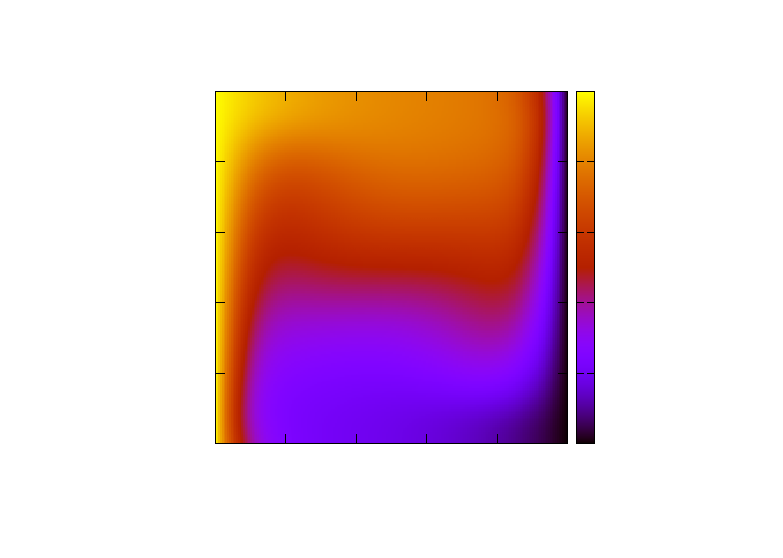
\includegraphics{Buoyancy/T5}}%
    \gplfronttext
  \end{picture}%
\endgroup
}
		\caption{$Ra=10^{5}$}
	\end{subfigure}%
	\begin{subfigure}{0.5\textwidth}
		\resizebox{1.4\textwidth}{!}{% GNUPLOT: LaTeX picture with Postscript
\begingroup
  \makeatletter
  \providecommand\color[2][]{%
    \GenericError{(gnuplot) \space\space\space\@spaces}{%
      Package color not loaded in conjunction with
      terminal option `colourtext'%
    }{See the gnuplot documentation for explanation.%
    }{Either use 'blacktext' in gnuplot or load the package
      color.sty in LaTeX.}%
    \renewcommand\color[2][]{}%
  }%
  \providecommand\includegraphics[2][]{%
    \GenericError{(gnuplot) \space\space\space\@spaces}{%
      Package graphicx or graphics not loaded%
    }{See the gnuplot documentation for explanation.%
    }{The gnuplot epslatex terminal needs graphicx.sty or graphics.sty.}%
    \renewcommand\includegraphics[2][]{}%
  }%
  \providecommand\rotatebox[2]{#2}%
  \@ifundefined{ifGPcolor}{%
    \newif\ifGPcolor
    \GPcolortrue
  }{}%
  \@ifundefined{ifGPblacktext}{%
    \newif\ifGPblacktext
    \GPblacktexttrue
  }{}%
  % define a \g@addto@macro without @ in the name:
  \let\gplgaddtomacro\g@addto@macro
  % define empty templates for all commands taking text:
  \gdef\gplbacktext{}%
  \gdef\gplfronttext{}%
  \makeatother
  \ifGPblacktext
    % no textcolor at all
    \def\colorrgb#1{}%
    \def\colorgray#1{}%
  \else
    % gray or color?
    \ifGPcolor
      \def\colorrgb#1{\color[rgb]{#1}}%
      \def\colorgray#1{\color[gray]{#1}}%
      \expandafter\def\csname LTw\endcsname{\color{white}}%
      \expandafter\def\csname LTb\endcsname{\color{black}}%
      \expandafter\def\csname LTa\endcsname{\color{black}}%
      \expandafter\def\csname LT0\endcsname{\color[rgb]{1,0,0}}%
      \expandafter\def\csname LT1\endcsname{\color[rgb]{0,1,0}}%
      \expandafter\def\csname LT2\endcsname{\color[rgb]{0,0,1}}%
      \expandafter\def\csname LT3\endcsname{\color[rgb]{1,0,1}}%
      \expandafter\def\csname LT4\endcsname{\color[rgb]{0,1,1}}%
      \expandafter\def\csname LT5\endcsname{\color[rgb]{1,1,0}}%
      \expandafter\def\csname LT6\endcsname{\color[rgb]{0,0,0}}%
      \expandafter\def\csname LT7\endcsname{\color[rgb]{1,0.3,0}}%
      \expandafter\def\csname LT8\endcsname{\color[rgb]{0.5,0.5,0.5}}%
    \else
      % gray
      \def\colorrgb#1{\color{black}}%
      \def\colorgray#1{\color[gray]{#1}}%
      \expandafter\def\csname LTw\endcsname{\color{white}}%
      \expandafter\def\csname LTb\endcsname{\color{black}}%
      \expandafter\def\csname LTa\endcsname{\color{black}}%
      \expandafter\def\csname LT0\endcsname{\color{black}}%
      \expandafter\def\csname LT1\endcsname{\color{black}}%
      \expandafter\def\csname LT2\endcsname{\color{black}}%
      \expandafter\def\csname LT3\endcsname{\color{black}}%
      \expandafter\def\csname LT4\endcsname{\color{black}}%
      \expandafter\def\csname LT5\endcsname{\color{black}}%
      \expandafter\def\csname LT6\endcsname{\color{black}}%
      \expandafter\def\csname LT7\endcsname{\color{black}}%
      \expandafter\def\csname LT8\endcsname{\color{black}}%
    \fi
  \fi
    \setlength{\unitlength}{0.0500bp}%
    \ifx\gptboxheight\undefined%
      \newlength{\gptboxheight}%
      \newlength{\gptboxwidth}%
      \newsavebox{\gptboxtext}%
    \fi%
    \setlength{\fboxrule}{0.5pt}%
    \setlength{\fboxsep}{1pt}%
\begin{picture}(7200.00,5040.00)%
    \gplgaddtomacro\gplbacktext{%
    }%
    \gplgaddtomacro\gplfronttext{%
      \put(1908,624){\makebox(0,0){\strut{}$0$}}%
      \put(2585,624){\makebox(0,0){\strut{}$0.2$}}%
      \put(3262,624){\makebox(0,0){\strut{}$0.4$}}%
      \put(3938,624){\makebox(0,0){\strut{}$0.6$}}%
      \put(4615,624){\makebox(0,0){\strut{}$0.8$}}%
      \put(5292,624){\makebox(0,0){\strut{}$1$}}%
      \put(1720,938){\makebox(0,0)[r]{\strut{}$0$}}%
      \put(1720,1615){\makebox(0,0)[r]{\strut{}$0.2$}}%
      \put(1720,2292){\makebox(0,0)[r]{\strut{}$0.4$}}%
      \put(1720,2968){\makebox(0,0)[r]{\strut{}$0.6$}}%
      \put(1720,3645){\makebox(0,0)[r]{\strut{}$0.8$}}%
      \put(1720,4322){\makebox(0,0)[r]{\strut{}$1$}}%
      \put(5678,938){\makebox(0,0)[l]{\strut{}$0$}}%
      \put(5678,1614){\makebox(0,0)[l]{\strut{}$0.2$}}%
      \put(5678,2291){\makebox(0,0)[l]{\strut{}$0.4$}}%
      \put(5678,2968){\makebox(0,0)[l]{\strut{}$0.6$}}%
      \put(5678,3645){\makebox(0,0)[l]{\strut{}$0.8$}}%
      \put(5678,4322){\makebox(0,0)[l]{\strut{}$1$}}%
    }%
    \gplbacktext
    \put(0,0){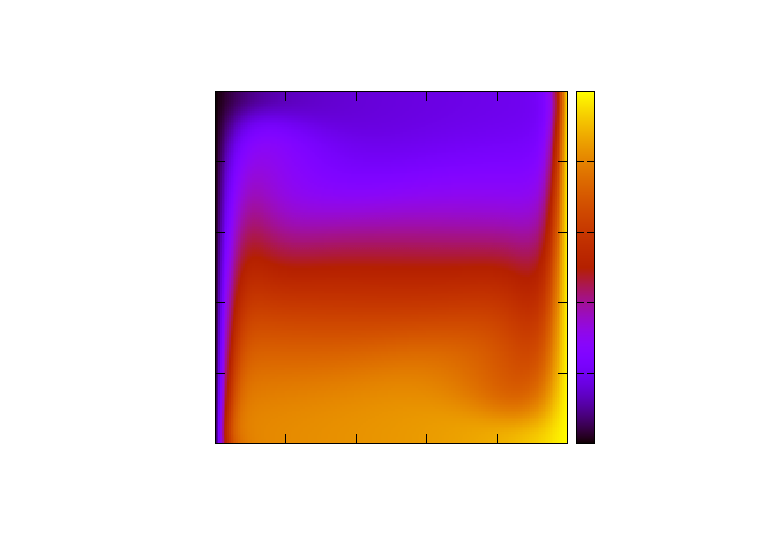
\includegraphics{Buoyancy/T6}}%
    \gplfronttext
  \end{picture}%
\endgroup
}
		\caption{$Ra=10^{6}$}
	\end{subfigure}
	\caption{Contour plots of the temperature}
	\label{TemperatureDiffHeated}
\end{figure}
In the temperature distribution (figure \ref{TemperatureDiffHeated}), there is a curve of the hot fluid (left wall) to the right in the top, whereas in the bottom the temperature decreases faster. This behaviour is explained because a higher temperature means a lower density, so the hot fluid tends to go on top. At low Ra, the temperature distribution is almost linear, like in conduction. But as Ra increases, the mentioned curve becomes more pronounced, until the highest Rayleigh numbers in which practically the half top of the cavity is hot and the half bottom is cold. This increase in Ra is like an increase in the volumetric thermal expansion coefficient, which means that density varies more with temperature. In other words, at very low Ra, the heat transfer is mainly by conduction, but as the Rayleigh number increases the differences in density become more important and the heat transport is by convection.

\begin{figure}[h]
	\begin{subfigure}{0.5\textwidth}
		\resizebox{1.4\textwidth}{!}{% GNUPLOT: LaTeX picture with Postscript
\begingroup
  \makeatletter
  \providecommand\color[2][]{%
    \GenericError{(gnuplot) \space\space\space\@spaces}{%
      Package color not loaded in conjunction with
      terminal option `colourtext'%
    }{See the gnuplot documentation for explanation.%
    }{Either use 'blacktext' in gnuplot or load the package
      color.sty in LaTeX.}%
    \renewcommand\color[2][]{}%
  }%
  \providecommand\includegraphics[2][]{%
    \GenericError{(gnuplot) \space\space\space\@spaces}{%
      Package graphicx or graphics not loaded%
    }{See the gnuplot documentation for explanation.%
    }{The gnuplot epslatex terminal needs graphicx.sty or graphics.sty.}%
    \renewcommand\includegraphics[2][]{}%
  }%
  \providecommand\rotatebox[2]{#2}%
  \@ifundefined{ifGPcolor}{%
    \newif\ifGPcolor
    \GPcolortrue
  }{}%
  \@ifundefined{ifGPblacktext}{%
    \newif\ifGPblacktext
    \GPblacktexttrue
  }{}%
  % define a \g@addto@macro without @ in the name:
  \let\gplgaddtomacro\g@addto@macro
  % define empty templates for all commands taking text:
  \gdef\gplbacktext{}%
  \gdef\gplfronttext{}%
  \makeatother
  \ifGPblacktext
    % no textcolor at all
    \def\colorrgb#1{}%
    \def\colorgray#1{}%
  \else
    % gray or color?
    \ifGPcolor
      \def\colorrgb#1{\color[rgb]{#1}}%
      \def\colorgray#1{\color[gray]{#1}}%
      \expandafter\def\csname LTw\endcsname{\color{white}}%
      \expandafter\def\csname LTb\endcsname{\color{black}}%
      \expandafter\def\csname LTa\endcsname{\color{black}}%
      \expandafter\def\csname LT0\endcsname{\color[rgb]{1,0,0}}%
      \expandafter\def\csname LT1\endcsname{\color[rgb]{0,1,0}}%
      \expandafter\def\csname LT2\endcsname{\color[rgb]{0,0,1}}%
      \expandafter\def\csname LT3\endcsname{\color[rgb]{1,0,1}}%
      \expandafter\def\csname LT4\endcsname{\color[rgb]{0,1,1}}%
      \expandafter\def\csname LT5\endcsname{\color[rgb]{1,1,0}}%
      \expandafter\def\csname LT6\endcsname{\color[rgb]{0,0,0}}%
      \expandafter\def\csname LT7\endcsname{\color[rgb]{1,0.3,0}}%
      \expandafter\def\csname LT8\endcsname{\color[rgb]{0.5,0.5,0.5}}%
    \else
      % gray
      \def\colorrgb#1{\color{black}}%
      \def\colorgray#1{\color[gray]{#1}}%
      \expandafter\def\csname LTw\endcsname{\color{white}}%
      \expandafter\def\csname LTb\endcsname{\color{black}}%
      \expandafter\def\csname LTa\endcsname{\color{black}}%
      \expandafter\def\csname LT0\endcsname{\color{black}}%
      \expandafter\def\csname LT1\endcsname{\color{black}}%
      \expandafter\def\csname LT2\endcsname{\color{black}}%
      \expandafter\def\csname LT3\endcsname{\color{black}}%
      \expandafter\def\csname LT4\endcsname{\color{black}}%
      \expandafter\def\csname LT5\endcsname{\color{black}}%
      \expandafter\def\csname LT6\endcsname{\color{black}}%
      \expandafter\def\csname LT7\endcsname{\color{black}}%
      \expandafter\def\csname LT8\endcsname{\color{black}}%
    \fi
  \fi
    \setlength{\unitlength}{0.0500bp}%
    \ifx\gptboxheight\undefined%
      \newlength{\gptboxheight}%
      \newlength{\gptboxwidth}%
      \newsavebox{\gptboxtext}%
    \fi%
    \setlength{\fboxrule}{0.5pt}%
    \setlength{\fboxsep}{1pt}%
\begin{picture}(7200.00,5040.00)%
    \gplgaddtomacro\gplbacktext{%
    }%
    \gplgaddtomacro\gplfronttext{%
      \put(1908,624){\makebox(0,0){\strut{}$0$}}%
      \put(2585,624){\makebox(0,0){\strut{}$0.2$}}%
      \put(3262,624){\makebox(0,0){\strut{}$0.4$}}%
      \put(3938,624){\makebox(0,0){\strut{}$0.6$}}%
      \put(4615,624){\makebox(0,0){\strut{}$0.8$}}%
      \put(5292,624){\makebox(0,0){\strut{}$1$}}%
      \put(1720,938){\makebox(0,0)[r]{\strut{}$0$}}%
      \put(1720,1615){\makebox(0,0)[r]{\strut{}$0.2$}}%
      \put(1720,2292){\makebox(0,0)[r]{\strut{}$0.4$}}%
      \put(1720,2968){\makebox(0,0)[r]{\strut{}$0.6$}}%
      \put(1720,3645){\makebox(0,0)[r]{\strut{}$0.8$}}%
      \put(1720,4322){\makebox(0,0)[r]{\strut{}$1$}}%
      \put(5678,938){\makebox(0,0)[l]{\strut{}$-4$}}%
      \put(5678,1361){\makebox(0,0)[l]{\strut{}$-3$}}%
      \put(5678,1784){\makebox(0,0)[l]{\strut{}$-2$}}%
      \put(5678,2207){\makebox(0,0)[l]{\strut{}$-1$}}%
      \put(5678,2630){\makebox(0,0)[l]{\strut{}$0$}}%
      \put(5678,3053){\makebox(0,0)[l]{\strut{}$1$}}%
      \put(5678,3476){\makebox(0,0)[l]{\strut{}$2$}}%
      \put(5678,3899){\makebox(0,0)[l]{\strut{}$3$}}%
      \put(5678,4322){\makebox(0,0)[l]{\strut{}$4$}}%
    }%
    \gplbacktext
    \put(0,0){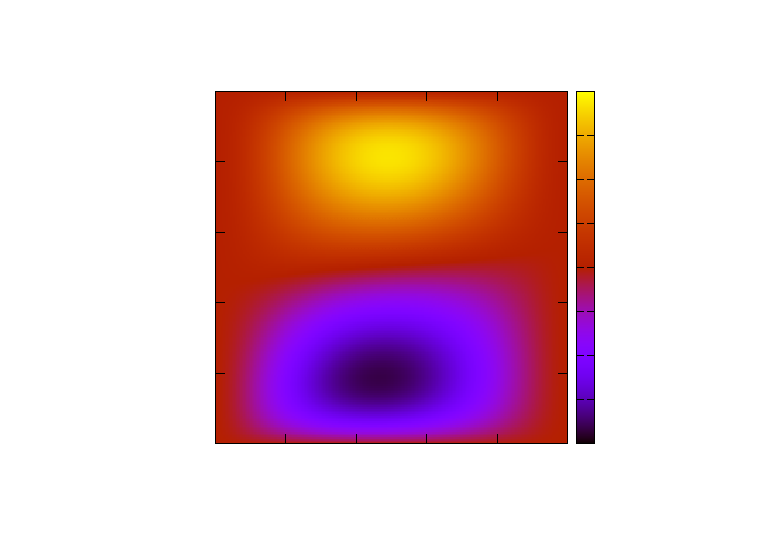
\includegraphics{Buoyancy/u3}}%
    \gplfronttext
  \end{picture}%
\endgroup
}
		\caption{$Ra=10^{3}$}
	\end{subfigure}%
	\begin{subfigure}{0.5\textwidth}
		\resizebox{1.4\textwidth}{!}{% GNUPLOT: LaTeX picture with Postscript
\begingroup
  \makeatletter
  \providecommand\color[2][]{%
    \GenericError{(gnuplot) \space\space\space\@spaces}{%
      Package color not loaded in conjunction with
      terminal option `colourtext'%
    }{See the gnuplot documentation for explanation.%
    }{Either use 'blacktext' in gnuplot or load the package
      color.sty in LaTeX.}%
    \renewcommand\color[2][]{}%
  }%
  \providecommand\includegraphics[2][]{%
    \GenericError{(gnuplot) \space\space\space\@spaces}{%
      Package graphicx or graphics not loaded%
    }{See the gnuplot documentation for explanation.%
    }{The gnuplot epslatex terminal needs graphicx.sty or graphics.sty.}%
    \renewcommand\includegraphics[2][]{}%
  }%
  \providecommand\rotatebox[2]{#2}%
  \@ifundefined{ifGPcolor}{%
    \newif\ifGPcolor
    \GPcolortrue
  }{}%
  \@ifundefined{ifGPblacktext}{%
    \newif\ifGPblacktext
    \GPblacktexttrue
  }{}%
  % define a \g@addto@macro without @ in the name:
  \let\gplgaddtomacro\g@addto@macro
  % define empty templates for all commands taking text:
  \gdef\gplbacktext{}%
  \gdef\gplfronttext{}%
  \makeatother
  \ifGPblacktext
    % no textcolor at all
    \def\colorrgb#1{}%
    \def\colorgray#1{}%
  \else
    % gray or color?
    \ifGPcolor
      \def\colorrgb#1{\color[rgb]{#1}}%
      \def\colorgray#1{\color[gray]{#1}}%
      \expandafter\def\csname LTw\endcsname{\color{white}}%
      \expandafter\def\csname LTb\endcsname{\color{black}}%
      \expandafter\def\csname LTa\endcsname{\color{black}}%
      \expandafter\def\csname LT0\endcsname{\color[rgb]{1,0,0}}%
      \expandafter\def\csname LT1\endcsname{\color[rgb]{0,1,0}}%
      \expandafter\def\csname LT2\endcsname{\color[rgb]{0,0,1}}%
      \expandafter\def\csname LT3\endcsname{\color[rgb]{1,0,1}}%
      \expandafter\def\csname LT4\endcsname{\color[rgb]{0,1,1}}%
      \expandafter\def\csname LT5\endcsname{\color[rgb]{1,1,0}}%
      \expandafter\def\csname LT6\endcsname{\color[rgb]{0,0,0}}%
      \expandafter\def\csname LT7\endcsname{\color[rgb]{1,0.3,0}}%
      \expandafter\def\csname LT8\endcsname{\color[rgb]{0.5,0.5,0.5}}%
    \else
      % gray
      \def\colorrgb#1{\color{black}}%
      \def\colorgray#1{\color[gray]{#1}}%
      \expandafter\def\csname LTw\endcsname{\color{white}}%
      \expandafter\def\csname LTb\endcsname{\color{black}}%
      \expandafter\def\csname LTa\endcsname{\color{black}}%
      \expandafter\def\csname LT0\endcsname{\color{black}}%
      \expandafter\def\csname LT1\endcsname{\color{black}}%
      \expandafter\def\csname LT2\endcsname{\color{black}}%
      \expandafter\def\csname LT3\endcsname{\color{black}}%
      \expandafter\def\csname LT4\endcsname{\color{black}}%
      \expandafter\def\csname LT5\endcsname{\color{black}}%
      \expandafter\def\csname LT6\endcsname{\color{black}}%
      \expandafter\def\csname LT7\endcsname{\color{black}}%
      \expandafter\def\csname LT8\endcsname{\color{black}}%
    \fi
  \fi
    \setlength{\unitlength}{0.0500bp}%
    \ifx\gptboxheight\undefined%
      \newlength{\gptboxheight}%
      \newlength{\gptboxwidth}%
      \newsavebox{\gptboxtext}%
    \fi%
    \setlength{\fboxrule}{0.5pt}%
    \setlength{\fboxsep}{1pt}%
\begin{picture}(7200.00,5040.00)%
    \gplgaddtomacro\gplbacktext{%
    }%
    \gplgaddtomacro\gplfronttext{%
      \put(1908,624){\makebox(0,0){\strut{}$0$}}%
      \put(2585,624){\makebox(0,0){\strut{}$0.2$}}%
      \put(3262,624){\makebox(0,0){\strut{}$0.4$}}%
      \put(3938,624){\makebox(0,0){\strut{}$0.6$}}%
      \put(4615,624){\makebox(0,0){\strut{}$0.8$}}%
      \put(5292,624){\makebox(0,0){\strut{}$1$}}%
      \put(1720,938){\makebox(0,0)[r]{\strut{}$0$}}%
      \put(1720,1615){\makebox(0,0)[r]{\strut{}$0.2$}}%
      \put(1720,2292){\makebox(0,0)[r]{\strut{}$0.4$}}%
      \put(1720,2968){\makebox(0,0)[r]{\strut{}$0.6$}}%
      \put(1720,3645){\makebox(0,0)[r]{\strut{}$0.8$}}%
      \put(1720,4322){\makebox(0,0)[r]{\strut{}$1$}}%
      \put(5678,938){\makebox(0,0)[l]{\strut{}$-20$}}%
      \put(5678,1361){\makebox(0,0)[l]{\strut{}$-15$}}%
      \put(5678,1784){\makebox(0,0)[l]{\strut{}$-10$}}%
      \put(5678,2207){\makebox(0,0)[l]{\strut{}$-5$}}%
      \put(5678,2630){\makebox(0,0)[l]{\strut{}$0$}}%
      \put(5678,3053){\makebox(0,0)[l]{\strut{}$5$}}%
      \put(5678,3476){\makebox(0,0)[l]{\strut{}$10$}}%
      \put(5678,3899){\makebox(0,0)[l]{\strut{}$15$}}%
      \put(5678,4322){\makebox(0,0)[l]{\strut{}$20$}}%
    }%
    \gplbacktext
    \put(0,0){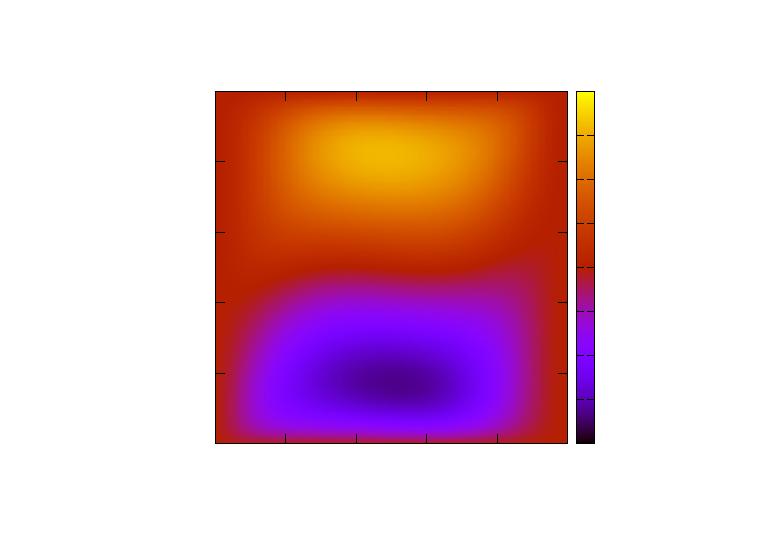
\includegraphics{Buoyancy/u4}}%
    \gplfronttext
  \end{picture}%
\endgroup
}
		\caption{$Ra=10^{4}$}
	\end{subfigure}
	\begin{subfigure}{0.5\textwidth}
		\resizebox{1.4\textwidth}{!}{% GNUPLOT: LaTeX picture with Postscript
\begingroup
  \makeatletter
  \providecommand\color[2][]{%
    \GenericError{(gnuplot) \space\space\space\@spaces}{%
      Package color not loaded in conjunction with
      terminal option `colourtext'%
    }{See the gnuplot documentation for explanation.%
    }{Either use 'blacktext' in gnuplot or load the package
      color.sty in LaTeX.}%
    \renewcommand\color[2][]{}%
  }%
  \providecommand\includegraphics[2][]{%
    \GenericError{(gnuplot) \space\space\space\@spaces}{%
      Package graphicx or graphics not loaded%
    }{See the gnuplot documentation for explanation.%
    }{The gnuplot epslatex terminal needs graphicx.sty or graphics.sty.}%
    \renewcommand\includegraphics[2][]{}%
  }%
  \providecommand\rotatebox[2]{#2}%
  \@ifundefined{ifGPcolor}{%
    \newif\ifGPcolor
    \GPcolortrue
  }{}%
  \@ifundefined{ifGPblacktext}{%
    \newif\ifGPblacktext
    \GPblacktexttrue
  }{}%
  % define a \g@addto@macro without @ in the name:
  \let\gplgaddtomacro\g@addto@macro
  % define empty templates for all commands taking text:
  \gdef\gplbacktext{}%
  \gdef\gplfronttext{}%
  \makeatother
  \ifGPblacktext
    % no textcolor at all
    \def\colorrgb#1{}%
    \def\colorgray#1{}%
  \else
    % gray or color?
    \ifGPcolor
      \def\colorrgb#1{\color[rgb]{#1}}%
      \def\colorgray#1{\color[gray]{#1}}%
      \expandafter\def\csname LTw\endcsname{\color{white}}%
      \expandafter\def\csname LTb\endcsname{\color{black}}%
      \expandafter\def\csname LTa\endcsname{\color{black}}%
      \expandafter\def\csname LT0\endcsname{\color[rgb]{1,0,0}}%
      \expandafter\def\csname LT1\endcsname{\color[rgb]{0,1,0}}%
      \expandafter\def\csname LT2\endcsname{\color[rgb]{0,0,1}}%
      \expandafter\def\csname LT3\endcsname{\color[rgb]{1,0,1}}%
      \expandafter\def\csname LT4\endcsname{\color[rgb]{0,1,1}}%
      \expandafter\def\csname LT5\endcsname{\color[rgb]{1,1,0}}%
      \expandafter\def\csname LT6\endcsname{\color[rgb]{0,0,0}}%
      \expandafter\def\csname LT7\endcsname{\color[rgb]{1,0.3,0}}%
      \expandafter\def\csname LT8\endcsname{\color[rgb]{0.5,0.5,0.5}}%
    \else
      % gray
      \def\colorrgb#1{\color{black}}%
      \def\colorgray#1{\color[gray]{#1}}%
      \expandafter\def\csname LTw\endcsname{\color{white}}%
      \expandafter\def\csname LTb\endcsname{\color{black}}%
      \expandafter\def\csname LTa\endcsname{\color{black}}%
      \expandafter\def\csname LT0\endcsname{\color{black}}%
      \expandafter\def\csname LT1\endcsname{\color{black}}%
      \expandafter\def\csname LT2\endcsname{\color{black}}%
      \expandafter\def\csname LT3\endcsname{\color{black}}%
      \expandafter\def\csname LT4\endcsname{\color{black}}%
      \expandafter\def\csname LT5\endcsname{\color{black}}%
      \expandafter\def\csname LT6\endcsname{\color{black}}%
      \expandafter\def\csname LT7\endcsname{\color{black}}%
      \expandafter\def\csname LT8\endcsname{\color{black}}%
    \fi
  \fi
    \setlength{\unitlength}{0.0500bp}%
    \ifx\gptboxheight\undefined%
      \newlength{\gptboxheight}%
      \newlength{\gptboxwidth}%
      \newsavebox{\gptboxtext}%
    \fi%
    \setlength{\fboxrule}{0.5pt}%
    \setlength{\fboxsep}{1pt}%
\begin{picture}(7200.00,5040.00)%
    \gplgaddtomacro\gplbacktext{%
    }%
    \gplgaddtomacro\gplfronttext{%
      \csname LTb\endcsname%
      \put(4374,4149){\makebox(0,0)[r]{\strut{}'u5.dat' using 1:2:3}}%
      \csname LTb\endcsname%
      \put(1908,624){\makebox(0,0){\strut{}$0$}}%
      \put(2585,624){\makebox(0,0){\strut{}$0.2$}}%
      \put(3262,624){\makebox(0,0){\strut{}$0.4$}}%
      \put(3938,624){\makebox(0,0){\strut{}$0.6$}}%
      \put(4615,624){\makebox(0,0){\strut{}$0.8$}}%
      \put(5292,624){\makebox(0,0){\strut{}$1$}}%
      \put(1720,938){\makebox(0,0)[r]{\strut{}$0$}}%
      \put(1720,1615){\makebox(0,0)[r]{\strut{}$0.2$}}%
      \put(1720,2292){\makebox(0,0)[r]{\strut{}$0.4$}}%
      \put(1720,2968){\makebox(0,0)[r]{\strut{}$0.6$}}%
      \put(1720,3645){\makebox(0,0)[r]{\strut{}$0.8$}}%
      \put(1720,4322){\makebox(0,0)[r]{\strut{}$1$}}%
      \put(5678,938){\makebox(0,0)[l]{\strut{}$-50$}}%
      \put(5678,1276){\makebox(0,0)[l]{\strut{}$-40$}}%
      \put(5678,1614){\makebox(0,0)[l]{\strut{}$-30$}}%
      \put(5678,1953){\makebox(0,0)[l]{\strut{}$-20$}}%
      \put(5678,2291){\makebox(0,0)[l]{\strut{}$-10$}}%
      \put(5678,2630){\makebox(0,0)[l]{\strut{}$0$}}%
      \put(5678,2968){\makebox(0,0)[l]{\strut{}$10$}}%
      \put(5678,3306){\makebox(0,0)[l]{\strut{}$20$}}%
      \put(5678,3645){\makebox(0,0)[l]{\strut{}$30$}}%
      \put(5678,3983){\makebox(0,0)[l]{\strut{}$40$}}%
      \put(5678,4322){\makebox(0,0)[l]{\strut{}$50$}}%
    }%
    \gplbacktext
    \put(0,0){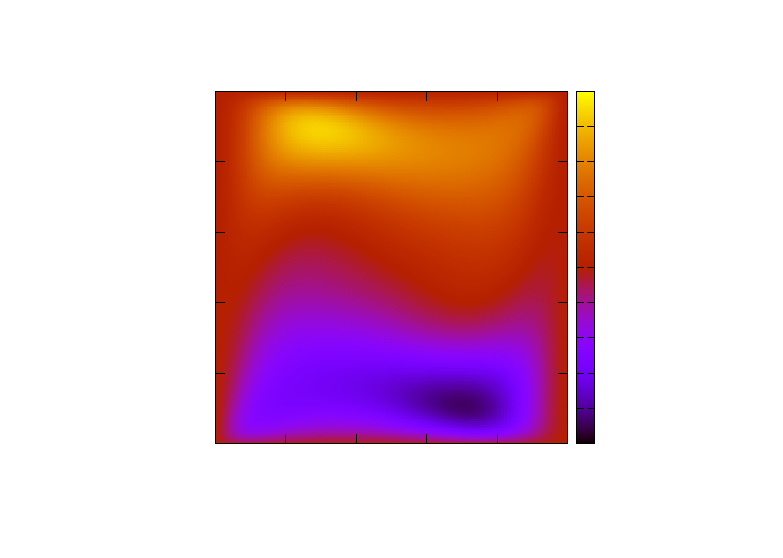
\includegraphics{Buoyancy/u5}}%
    \gplfronttext
  \end{picture}%
\endgroup
}
		\caption{$Ra=10^{5}$}
	\end{subfigure}%
	\begin{subfigure}{0.5\textwidth}
		\resizebox{1.4\textwidth}{!}{% GNUPLOT: LaTeX picture with Postscript
\begingroup
  \makeatletter
  \providecommand\color[2][]{%
    \GenericError{(gnuplot) \space\space\space\@spaces}{%
      Package color not loaded in conjunction with
      terminal option `colourtext'%
    }{See the gnuplot documentation for explanation.%
    }{Either use 'blacktext' in gnuplot or load the package
      color.sty in LaTeX.}%
    \renewcommand\color[2][]{}%
  }%
  \providecommand\includegraphics[2][]{%
    \GenericError{(gnuplot) \space\space\space\@spaces}{%
      Package graphicx or graphics not loaded%
    }{See the gnuplot documentation for explanation.%
    }{The gnuplot epslatex terminal needs graphicx.sty or graphics.sty.}%
    \renewcommand\includegraphics[2][]{}%
  }%
  \providecommand\rotatebox[2]{#2}%
  \@ifundefined{ifGPcolor}{%
    \newif\ifGPcolor
    \GPcolortrue
  }{}%
  \@ifundefined{ifGPblacktext}{%
    \newif\ifGPblacktext
    \GPblacktexttrue
  }{}%
  % define a \g@addto@macro without @ in the name:
  \let\gplgaddtomacro\g@addto@macro
  % define empty templates for all commands taking text:
  \gdef\gplbacktext{}%
  \gdef\gplfronttext{}%
  \makeatother
  \ifGPblacktext
    % no textcolor at all
    \def\colorrgb#1{}%
    \def\colorgray#1{}%
  \else
    % gray or color?
    \ifGPcolor
      \def\colorrgb#1{\color[rgb]{#1}}%
      \def\colorgray#1{\color[gray]{#1}}%
      \expandafter\def\csname LTw\endcsname{\color{white}}%
      \expandafter\def\csname LTb\endcsname{\color{black}}%
      \expandafter\def\csname LTa\endcsname{\color{black}}%
      \expandafter\def\csname LT0\endcsname{\color[rgb]{1,0,0}}%
      \expandafter\def\csname LT1\endcsname{\color[rgb]{0,1,0}}%
      \expandafter\def\csname LT2\endcsname{\color[rgb]{0,0,1}}%
      \expandafter\def\csname LT3\endcsname{\color[rgb]{1,0,1}}%
      \expandafter\def\csname LT4\endcsname{\color[rgb]{0,1,1}}%
      \expandafter\def\csname LT5\endcsname{\color[rgb]{1,1,0}}%
      \expandafter\def\csname LT6\endcsname{\color[rgb]{0,0,0}}%
      \expandafter\def\csname LT7\endcsname{\color[rgb]{1,0.3,0}}%
      \expandafter\def\csname LT8\endcsname{\color[rgb]{0.5,0.5,0.5}}%
    \else
      % gray
      \def\colorrgb#1{\color{black}}%
      \def\colorgray#1{\color[gray]{#1}}%
      \expandafter\def\csname LTw\endcsname{\color{white}}%
      \expandafter\def\csname LTb\endcsname{\color{black}}%
      \expandafter\def\csname LTa\endcsname{\color{black}}%
      \expandafter\def\csname LT0\endcsname{\color{black}}%
      \expandafter\def\csname LT1\endcsname{\color{black}}%
      \expandafter\def\csname LT2\endcsname{\color{black}}%
      \expandafter\def\csname LT3\endcsname{\color{black}}%
      \expandafter\def\csname LT4\endcsname{\color{black}}%
      \expandafter\def\csname LT5\endcsname{\color{black}}%
      \expandafter\def\csname LT6\endcsname{\color{black}}%
      \expandafter\def\csname LT7\endcsname{\color{black}}%
      \expandafter\def\csname LT8\endcsname{\color{black}}%
    \fi
  \fi
    \setlength{\unitlength}{0.0500bp}%
    \ifx\gptboxheight\undefined%
      \newlength{\gptboxheight}%
      \newlength{\gptboxwidth}%
      \newsavebox{\gptboxtext}%
    \fi%
    \setlength{\fboxrule}{0.5pt}%
    \setlength{\fboxsep}{1pt}%
\begin{picture}(7200.00,5040.00)%
    \gplgaddtomacro\gplbacktext{%
    }%
    \gplgaddtomacro\gplfronttext{%
      \csname LTb\endcsname%
      \put(4374,4149){\makebox(0,0)[r]{\strut{}'u6.dat' using 1:2:3}}%
      \csname LTb\endcsname%
      \put(1908,624){\makebox(0,0){\strut{}$0$}}%
      \put(2585,624){\makebox(0,0){\strut{}$0.2$}}%
      \put(3262,624){\makebox(0,0){\strut{}$0.4$}}%
      \put(3938,624){\makebox(0,0){\strut{}$0.6$}}%
      \put(4615,624){\makebox(0,0){\strut{}$0.8$}}%
      \put(5292,624){\makebox(0,0){\strut{}$1$}}%
      \put(1720,938){\makebox(0,0)[r]{\strut{}$0$}}%
      \put(1720,1615){\makebox(0,0)[r]{\strut{}$0.2$}}%
      \put(1720,2292){\makebox(0,0)[r]{\strut{}$0.4$}}%
      \put(1720,2968){\makebox(0,0)[r]{\strut{}$0.6$}}%
      \put(1720,3645){\makebox(0,0)[r]{\strut{}$0.8$}}%
      \put(1720,4322){\makebox(0,0)[r]{\strut{}$1$}}%
      \put(5678,938){\makebox(0,0)[l]{\strut{}$-150$}}%
      \put(5678,1502){\makebox(0,0)[l]{\strut{}$-100$}}%
      \put(5678,2066){\makebox(0,0)[l]{\strut{}$-50$}}%
      \put(5678,2630){\makebox(0,0)[l]{\strut{}$0$}}%
      \put(5678,3194){\makebox(0,0)[l]{\strut{}$50$}}%
      \put(5678,3758){\makebox(0,0)[l]{\strut{}$100$}}%
      \put(5678,4322){\makebox(0,0)[l]{\strut{}$150$}}%
    }%
    \gplbacktext
    \put(0,0){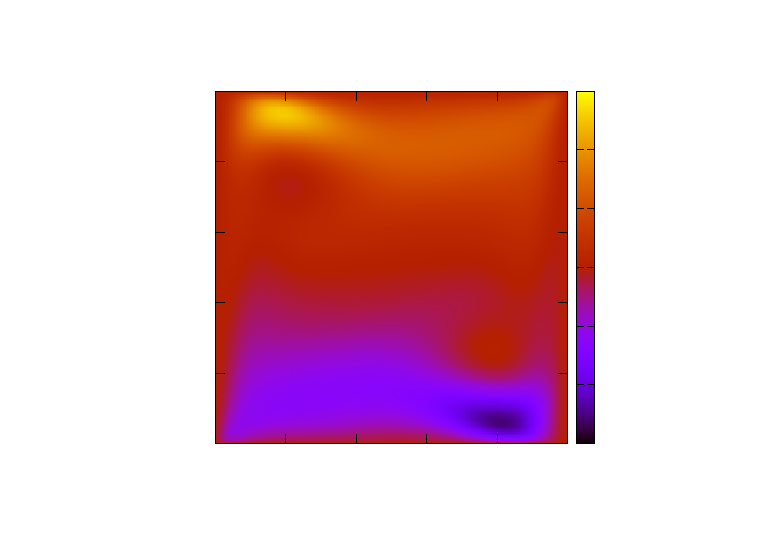
\includegraphics{Buoyancy/u6}}%
    \gplfronttext
  \end{picture}%
\endgroup
}
		\caption{$Ra=10^{6}$}
	\end{subfigure}
	\caption{Contour plots of the horizontal velocity}
	\label{uplotDiffHeated}
\end{figure}
\begin{figure}[h!]
	\begin{subfigure}{0.5\textwidth}
		\resizebox{1.4\textwidth}{!}{% GNUPLOT: LaTeX picture with Postscript
\begingroup
  \makeatletter
  \providecommand\color[2][]{%
    \GenericError{(gnuplot) \space\space\space\@spaces}{%
      Package color not loaded in conjunction with
      terminal option `colourtext'%
    }{See the gnuplot documentation for explanation.%
    }{Either use 'blacktext' in gnuplot or load the package
      color.sty in LaTeX.}%
    \renewcommand\color[2][]{}%
  }%
  \providecommand\includegraphics[2][]{%
    \GenericError{(gnuplot) \space\space\space\@spaces}{%
      Package graphicx or graphics not loaded%
    }{See the gnuplot documentation for explanation.%
    }{The gnuplot epslatex terminal needs graphicx.sty or graphics.sty.}%
    \renewcommand\includegraphics[2][]{}%
  }%
  \providecommand\rotatebox[2]{#2}%
  \@ifundefined{ifGPcolor}{%
    \newif\ifGPcolor
    \GPcolortrue
  }{}%
  \@ifundefined{ifGPblacktext}{%
    \newif\ifGPblacktext
    \GPblacktexttrue
  }{}%
  % define a \g@addto@macro without @ in the name:
  \let\gplgaddtomacro\g@addto@macro
  % define empty templates for all commands taking text:
  \gdef\gplbacktext{}%
  \gdef\gplfronttext{}%
  \makeatother
  \ifGPblacktext
    % no textcolor at all
    \def\colorrgb#1{}%
    \def\colorgray#1{}%
  \else
    % gray or color?
    \ifGPcolor
      \def\colorrgb#1{\color[rgb]{#1}}%
      \def\colorgray#1{\color[gray]{#1}}%
      \expandafter\def\csname LTw\endcsname{\color{white}}%
      \expandafter\def\csname LTb\endcsname{\color{black}}%
      \expandafter\def\csname LTa\endcsname{\color{black}}%
      \expandafter\def\csname LT0\endcsname{\color[rgb]{1,0,0}}%
      \expandafter\def\csname LT1\endcsname{\color[rgb]{0,1,0}}%
      \expandafter\def\csname LT2\endcsname{\color[rgb]{0,0,1}}%
      \expandafter\def\csname LT3\endcsname{\color[rgb]{1,0,1}}%
      \expandafter\def\csname LT4\endcsname{\color[rgb]{0,1,1}}%
      \expandafter\def\csname LT5\endcsname{\color[rgb]{1,1,0}}%
      \expandafter\def\csname LT6\endcsname{\color[rgb]{0,0,0}}%
      \expandafter\def\csname LT7\endcsname{\color[rgb]{1,0.3,0}}%
      \expandafter\def\csname LT8\endcsname{\color[rgb]{0.5,0.5,0.5}}%
    \else
      % gray
      \def\colorrgb#1{\color{black}}%
      \def\colorgray#1{\color[gray]{#1}}%
      \expandafter\def\csname LTw\endcsname{\color{white}}%
      \expandafter\def\csname LTb\endcsname{\color{black}}%
      \expandafter\def\csname LTa\endcsname{\color{black}}%
      \expandafter\def\csname LT0\endcsname{\color{black}}%
      \expandafter\def\csname LT1\endcsname{\color{black}}%
      \expandafter\def\csname LT2\endcsname{\color{black}}%
      \expandafter\def\csname LT3\endcsname{\color{black}}%
      \expandafter\def\csname LT4\endcsname{\color{black}}%
      \expandafter\def\csname LT5\endcsname{\color{black}}%
      \expandafter\def\csname LT6\endcsname{\color{black}}%
      \expandafter\def\csname LT7\endcsname{\color{black}}%
      \expandafter\def\csname LT8\endcsname{\color{black}}%
    \fi
  \fi
    \setlength{\unitlength}{0.0500bp}%
    \ifx\gptboxheight\undefined%
      \newlength{\gptboxheight}%
      \newlength{\gptboxwidth}%
      \newsavebox{\gptboxtext}%
    \fi%
    \setlength{\fboxrule}{0.5pt}%
    \setlength{\fboxsep}{1pt}%
\begin{picture}(7200.00,5040.00)%
    \gplgaddtomacro\gplbacktext{%
    }%
    \gplgaddtomacro\gplfronttext{%
      \csname LTb\endcsname%
      \put(4374,4149){\makebox(0,0)[r]{\strut{}'v3.dat' using 1:2:3}}%
      \csname LTb\endcsname%
      \put(1908,624){\makebox(0,0){\strut{}$0$}}%
      \put(2585,624){\makebox(0,0){\strut{}$0.2$}}%
      \put(3262,624){\makebox(0,0){\strut{}$0.4$}}%
      \put(3938,624){\makebox(0,0){\strut{}$0.6$}}%
      \put(4615,624){\makebox(0,0){\strut{}$0.8$}}%
      \put(5292,624){\makebox(0,0){\strut{}$1$}}%
      \put(1720,938){\makebox(0,0)[r]{\strut{}$0$}}%
      \put(1720,1615){\makebox(0,0)[r]{\strut{}$0.2$}}%
      \put(1720,2292){\makebox(0,0)[r]{\strut{}$0.4$}}%
      \put(1720,2968){\makebox(0,0)[r]{\strut{}$0.6$}}%
      \put(1720,3645){\makebox(0,0)[r]{\strut{}$0.8$}}%
      \put(1720,4322){\makebox(0,0)[r]{\strut{}$1$}}%
      \put(5678,938){\makebox(0,0)[l]{\strut{}$-5$}}%
      \put(5678,1314){\makebox(0,0)[l]{\strut{}$-4$}}%
      \put(5678,1690){\makebox(0,0)[l]{\strut{}$-3$}}%
      \put(5678,2066){\makebox(0,0)[l]{\strut{}$-2$}}%
      \put(5678,2442){\makebox(0,0)[l]{\strut{}$-1$}}%
      \put(5678,2818){\makebox(0,0)[l]{\strut{}$0$}}%
      \put(5678,3194){\makebox(0,0)[l]{\strut{}$1$}}%
      \put(5678,3570){\makebox(0,0)[l]{\strut{}$2$}}%
      \put(5678,3946){\makebox(0,0)[l]{\strut{}$3$}}%
      \put(5678,4322){\makebox(0,0)[l]{\strut{}$4$}}%
    }%
    \gplbacktext
    \put(0,0){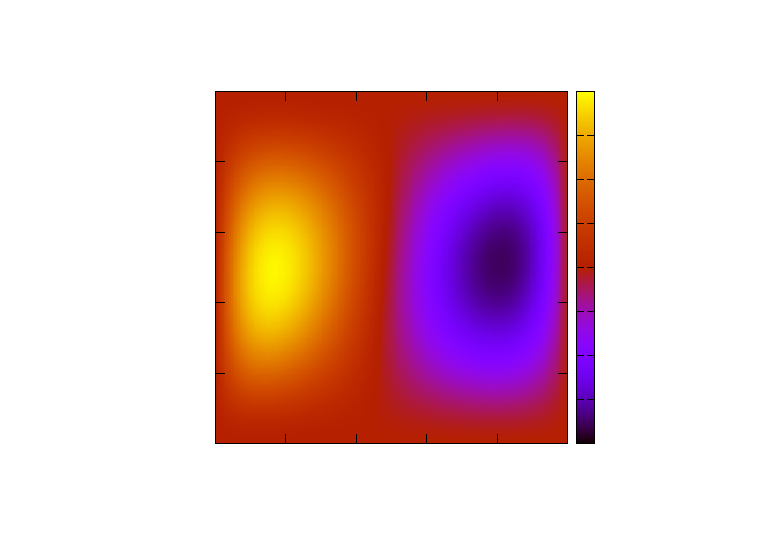
\includegraphics{Buoyancy/v3}}%
    \gplfronttext
  \end{picture}%
\endgroup
}
		\caption{$Ra=10^{3}$}
	\end{subfigure}%
	\begin{subfigure}{0.5\textwidth}
		\resizebox{1.4\textwidth}{!}{% GNUPLOT: LaTeX picture with Postscript
\begingroup
  \makeatletter
  \providecommand\color[2][]{%
    \GenericError{(gnuplot) \space\space\space\@spaces}{%
      Package color not loaded in conjunction with
      terminal option `colourtext'%
    }{See the gnuplot documentation for explanation.%
    }{Either use 'blacktext' in gnuplot or load the package
      color.sty in LaTeX.}%
    \renewcommand\color[2][]{}%
  }%
  \providecommand\includegraphics[2][]{%
    \GenericError{(gnuplot) \space\space\space\@spaces}{%
      Package graphicx or graphics not loaded%
    }{See the gnuplot documentation for explanation.%
    }{The gnuplot epslatex terminal needs graphicx.sty or graphics.sty.}%
    \renewcommand\includegraphics[2][]{}%
  }%
  \providecommand\rotatebox[2]{#2}%
  \@ifundefined{ifGPcolor}{%
    \newif\ifGPcolor
    \GPcolortrue
  }{}%
  \@ifundefined{ifGPblacktext}{%
    \newif\ifGPblacktext
    \GPblacktexttrue
  }{}%
  % define a \g@addto@macro without @ in the name:
  \let\gplgaddtomacro\g@addto@macro
  % define empty templates for all commands taking text:
  \gdef\gplbacktext{}%
  \gdef\gplfronttext{}%
  \makeatother
  \ifGPblacktext
    % no textcolor at all
    \def\colorrgb#1{}%
    \def\colorgray#1{}%
  \else
    % gray or color?
    \ifGPcolor
      \def\colorrgb#1{\color[rgb]{#1}}%
      \def\colorgray#1{\color[gray]{#1}}%
      \expandafter\def\csname LTw\endcsname{\color{white}}%
      \expandafter\def\csname LTb\endcsname{\color{black}}%
      \expandafter\def\csname LTa\endcsname{\color{black}}%
      \expandafter\def\csname LT0\endcsname{\color[rgb]{1,0,0}}%
      \expandafter\def\csname LT1\endcsname{\color[rgb]{0,1,0}}%
      \expandafter\def\csname LT2\endcsname{\color[rgb]{0,0,1}}%
      \expandafter\def\csname LT3\endcsname{\color[rgb]{1,0,1}}%
      \expandafter\def\csname LT4\endcsname{\color[rgb]{0,1,1}}%
      \expandafter\def\csname LT5\endcsname{\color[rgb]{1,1,0}}%
      \expandafter\def\csname LT6\endcsname{\color[rgb]{0,0,0}}%
      \expandafter\def\csname LT7\endcsname{\color[rgb]{1,0.3,0}}%
      \expandafter\def\csname LT8\endcsname{\color[rgb]{0.5,0.5,0.5}}%
    \else
      % gray
      \def\colorrgb#1{\color{black}}%
      \def\colorgray#1{\color[gray]{#1}}%
      \expandafter\def\csname LTw\endcsname{\color{white}}%
      \expandafter\def\csname LTb\endcsname{\color{black}}%
      \expandafter\def\csname LTa\endcsname{\color{black}}%
      \expandafter\def\csname LT0\endcsname{\color{black}}%
      \expandafter\def\csname LT1\endcsname{\color{black}}%
      \expandafter\def\csname LT2\endcsname{\color{black}}%
      \expandafter\def\csname LT3\endcsname{\color{black}}%
      \expandafter\def\csname LT4\endcsname{\color{black}}%
      \expandafter\def\csname LT5\endcsname{\color{black}}%
      \expandafter\def\csname LT6\endcsname{\color{black}}%
      \expandafter\def\csname LT7\endcsname{\color{black}}%
      \expandafter\def\csname LT8\endcsname{\color{black}}%
    \fi
  \fi
    \setlength{\unitlength}{0.0500bp}%
    \ifx\gptboxheight\undefined%
      \newlength{\gptboxheight}%
      \newlength{\gptboxwidth}%
      \newsavebox{\gptboxtext}%
    \fi%
    \setlength{\fboxrule}{0.5pt}%
    \setlength{\fboxsep}{1pt}%
\begin{picture}(7200.00,5040.00)%
    \gplgaddtomacro\gplbacktext{%
    }%
    \gplgaddtomacro\gplfronttext{%
      \put(1908,624){\makebox(0,0){\strut{}$0$}}%
      \put(2585,624){\makebox(0,0){\strut{}$0.2$}}%
      \put(3262,624){\makebox(0,0){\strut{}$0.4$}}%
      \put(3938,624){\makebox(0,0){\strut{}$0.6$}}%
      \put(4615,624){\makebox(0,0){\strut{}$0.8$}}%
      \put(5292,624){\makebox(0,0){\strut{}$1$}}%
      \put(1720,938){\makebox(0,0)[r]{\strut{}$0$}}%
      \put(1720,1615){\makebox(0,0)[r]{\strut{}$0.2$}}%
      \put(1720,2292){\makebox(0,0)[r]{\strut{}$0.4$}}%
      \put(1720,2968){\makebox(0,0)[r]{\strut{}$0.6$}}%
      \put(1720,3645){\makebox(0,0)[r]{\strut{}$0.8$}}%
      \put(1720,4322){\makebox(0,0)[r]{\strut{}$1$}}%
      \put(5678,938){\makebox(0,0)[l]{\strut{}$-20$}}%
      \put(5678,1361){\makebox(0,0)[l]{\strut{}$-15$}}%
      \put(5678,1784){\makebox(0,0)[l]{\strut{}$-10$}}%
      \put(5678,2207){\makebox(0,0)[l]{\strut{}$-5$}}%
      \put(5678,2630){\makebox(0,0)[l]{\strut{}$0$}}%
      \put(5678,3053){\makebox(0,0)[l]{\strut{}$5$}}%
      \put(5678,3476){\makebox(0,0)[l]{\strut{}$10$}}%
      \put(5678,3899){\makebox(0,0)[l]{\strut{}$15$}}%
      \put(5678,4322){\makebox(0,0)[l]{\strut{}$20$}}%
    }%
    \gplbacktext
    \put(0,0){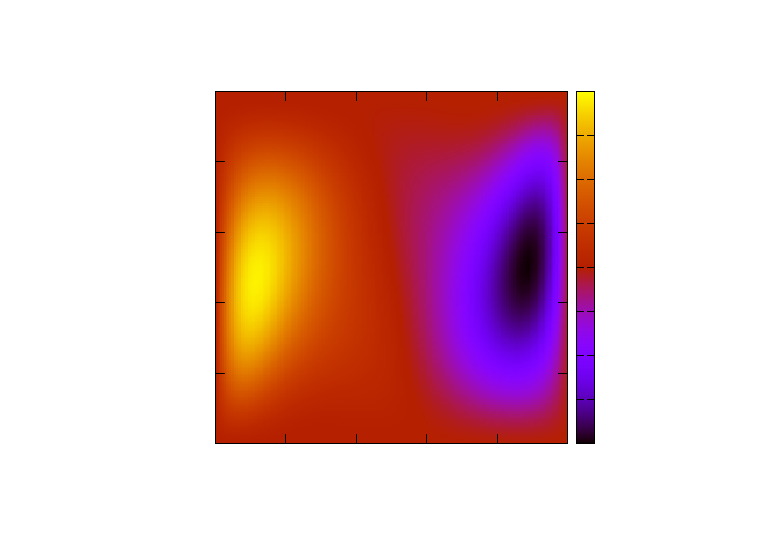
\includegraphics{Buoyancy/v4}}%
    \gplfronttext
  \end{picture}%
\endgroup
}
		\caption{$Ra=10^{4}$}
	\end{subfigure}
	\begin{subfigure}{0.5\textwidth}
		\resizebox{1.4\textwidth}{!}{% GNUPLOT: LaTeX picture with Postscript
\begingroup
  \makeatletter
  \providecommand\color[2][]{%
    \GenericError{(gnuplot) \space\space\space\@spaces}{%
      Package color not loaded in conjunction with
      terminal option `colourtext'%
    }{See the gnuplot documentation for explanation.%
    }{Either use 'blacktext' in gnuplot or load the package
      color.sty in LaTeX.}%
    \renewcommand\color[2][]{}%
  }%
  \providecommand\includegraphics[2][]{%
    \GenericError{(gnuplot) \space\space\space\@spaces}{%
      Package graphicx or graphics not loaded%
    }{See the gnuplot documentation for explanation.%
    }{The gnuplot epslatex terminal needs graphicx.sty or graphics.sty.}%
    \renewcommand\includegraphics[2][]{}%
  }%
  \providecommand\rotatebox[2]{#2}%
  \@ifundefined{ifGPcolor}{%
    \newif\ifGPcolor
    \GPcolortrue
  }{}%
  \@ifundefined{ifGPblacktext}{%
    \newif\ifGPblacktext
    \GPblacktexttrue
  }{}%
  % define a \g@addto@macro without @ in the name:
  \let\gplgaddtomacro\g@addto@macro
  % define empty templates for all commands taking text:
  \gdef\gplbacktext{}%
  \gdef\gplfronttext{}%
  \makeatother
  \ifGPblacktext
    % no textcolor at all
    \def\colorrgb#1{}%
    \def\colorgray#1{}%
  \else
    % gray or color?
    \ifGPcolor
      \def\colorrgb#1{\color[rgb]{#1}}%
      \def\colorgray#1{\color[gray]{#1}}%
      \expandafter\def\csname LTw\endcsname{\color{white}}%
      \expandafter\def\csname LTb\endcsname{\color{black}}%
      \expandafter\def\csname LTa\endcsname{\color{black}}%
      \expandafter\def\csname LT0\endcsname{\color[rgb]{1,0,0}}%
      \expandafter\def\csname LT1\endcsname{\color[rgb]{0,1,0}}%
      \expandafter\def\csname LT2\endcsname{\color[rgb]{0,0,1}}%
      \expandafter\def\csname LT3\endcsname{\color[rgb]{1,0,1}}%
      \expandafter\def\csname LT4\endcsname{\color[rgb]{0,1,1}}%
      \expandafter\def\csname LT5\endcsname{\color[rgb]{1,1,0}}%
      \expandafter\def\csname LT6\endcsname{\color[rgb]{0,0,0}}%
      \expandafter\def\csname LT7\endcsname{\color[rgb]{1,0.3,0}}%
      \expandafter\def\csname LT8\endcsname{\color[rgb]{0.5,0.5,0.5}}%
    \else
      % gray
      \def\colorrgb#1{\color{black}}%
      \def\colorgray#1{\color[gray]{#1}}%
      \expandafter\def\csname LTw\endcsname{\color{white}}%
      \expandafter\def\csname LTb\endcsname{\color{black}}%
      \expandafter\def\csname LTa\endcsname{\color{black}}%
      \expandafter\def\csname LT0\endcsname{\color{black}}%
      \expandafter\def\csname LT1\endcsname{\color{black}}%
      \expandafter\def\csname LT2\endcsname{\color{black}}%
      \expandafter\def\csname LT3\endcsname{\color{black}}%
      \expandafter\def\csname LT4\endcsname{\color{black}}%
      \expandafter\def\csname LT5\endcsname{\color{black}}%
      \expandafter\def\csname LT6\endcsname{\color{black}}%
      \expandafter\def\csname LT7\endcsname{\color{black}}%
      \expandafter\def\csname LT8\endcsname{\color{black}}%
    \fi
  \fi
    \setlength{\unitlength}{0.0500bp}%
    \ifx\gptboxheight\undefined%
      \newlength{\gptboxheight}%
      \newlength{\gptboxwidth}%
      \newsavebox{\gptboxtext}%
    \fi%
    \setlength{\fboxrule}{0.5pt}%
    \setlength{\fboxsep}{1pt}%
\begin{picture}(7200.00,5040.00)%
    \gplgaddtomacro\gplbacktext{%
    }%
    \gplgaddtomacro\gplfronttext{%
      \csname LTb\endcsname%
      \put(4374,4149){\makebox(0,0)[r]{\strut{}'v5.dat' using 1:2:3}}%
      \csname LTb\endcsname%
      \put(1908,624){\makebox(0,0){\strut{}$0$}}%
      \put(2585,624){\makebox(0,0){\strut{}$0.2$}}%
      \put(3262,624){\makebox(0,0){\strut{}$0.4$}}%
      \put(3938,624){\makebox(0,0){\strut{}$0.6$}}%
      \put(4615,624){\makebox(0,0){\strut{}$0.8$}}%
      \put(5292,624){\makebox(0,0){\strut{}$1$}}%
      \put(1720,938){\makebox(0,0)[r]{\strut{}$0$}}%
      \put(1720,1615){\makebox(0,0)[r]{\strut{}$0.2$}}%
      \put(1720,2292){\makebox(0,0)[r]{\strut{}$0.4$}}%
      \put(1720,2968){\makebox(0,0)[r]{\strut{}$0.6$}}%
      \put(1720,3645){\makebox(0,0)[r]{\strut{}$0.8$}}%
      \put(1720,4322){\makebox(0,0)[r]{\strut{}$1$}}%
      \put(5678,938){\makebox(0,0)[l]{\strut{}$-80$}}%
      \put(5678,1361){\makebox(0,0)[l]{\strut{}$-60$}}%
      \put(5678,1784){\makebox(0,0)[l]{\strut{}$-40$}}%
      \put(5678,2207){\makebox(0,0)[l]{\strut{}$-20$}}%
      \put(5678,2630){\makebox(0,0)[l]{\strut{}$0$}}%
      \put(5678,3053){\makebox(0,0)[l]{\strut{}$20$}}%
      \put(5678,3476){\makebox(0,0)[l]{\strut{}$40$}}%
      \put(5678,3899){\makebox(0,0)[l]{\strut{}$60$}}%
      \put(5678,4322){\makebox(0,0)[l]{\strut{}$80$}}%
    }%
    \gplbacktext
    \put(0,0){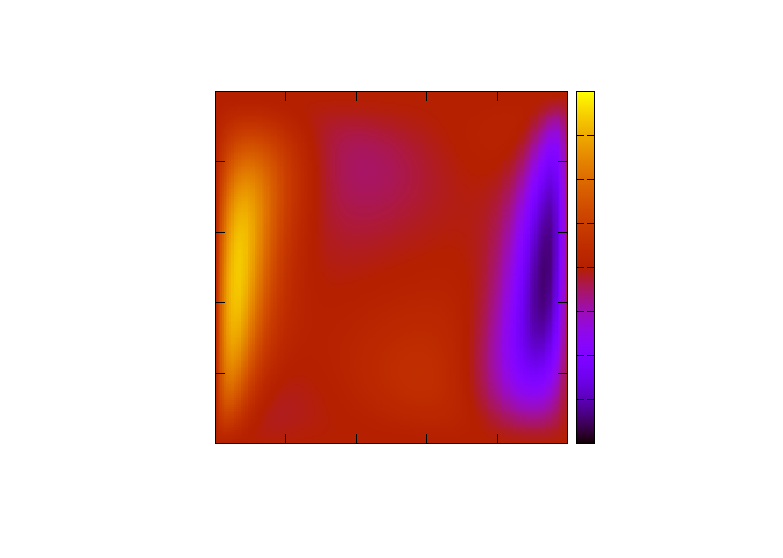
\includegraphics{Buoyancy/v5}}%
    \gplfronttext
  \end{picture}%
\endgroup
}
		\caption{$Ra=10^{5}$}
		\label{vplotRa5}
	\end{subfigure}%
	\begin{subfigure}{0.5\textwidth}
		\resizebox{1.4\textwidth}{!}{% GNUPLOT: LaTeX picture with Postscript
\begingroup
  \makeatletter
  \providecommand\color[2][]{%
    \GenericError{(gnuplot) \space\space\space\@spaces}{%
      Package color not loaded in conjunction with
      terminal option `colourtext'%
    }{See the gnuplot documentation for explanation.%
    }{Either use 'blacktext' in gnuplot or load the package
      color.sty in LaTeX.}%
    \renewcommand\color[2][]{}%
  }%
  \providecommand\includegraphics[2][]{%
    \GenericError{(gnuplot) \space\space\space\@spaces}{%
      Package graphicx or graphics not loaded%
    }{See the gnuplot documentation for explanation.%
    }{The gnuplot epslatex terminal needs graphicx.sty or graphics.sty.}%
    \renewcommand\includegraphics[2][]{}%
  }%
  \providecommand\rotatebox[2]{#2}%
  \@ifundefined{ifGPcolor}{%
    \newif\ifGPcolor
    \GPcolortrue
  }{}%
  \@ifundefined{ifGPblacktext}{%
    \newif\ifGPblacktext
    \GPblacktexttrue
  }{}%
  % define a \g@addto@macro without @ in the name:
  \let\gplgaddtomacro\g@addto@macro
  % define empty templates for all commands taking text:
  \gdef\gplbacktext{}%
  \gdef\gplfronttext{}%
  \makeatother
  \ifGPblacktext
    % no textcolor at all
    \def\colorrgb#1{}%
    \def\colorgray#1{}%
  \else
    % gray or color?
    \ifGPcolor
      \def\colorrgb#1{\color[rgb]{#1}}%
      \def\colorgray#1{\color[gray]{#1}}%
      \expandafter\def\csname LTw\endcsname{\color{white}}%
      \expandafter\def\csname LTb\endcsname{\color{black}}%
      \expandafter\def\csname LTa\endcsname{\color{black}}%
      \expandafter\def\csname LT0\endcsname{\color[rgb]{1,0,0}}%
      \expandafter\def\csname LT1\endcsname{\color[rgb]{0,1,0}}%
      \expandafter\def\csname LT2\endcsname{\color[rgb]{0,0,1}}%
      \expandafter\def\csname LT3\endcsname{\color[rgb]{1,0,1}}%
      \expandafter\def\csname LT4\endcsname{\color[rgb]{0,1,1}}%
      \expandafter\def\csname LT5\endcsname{\color[rgb]{1,1,0}}%
      \expandafter\def\csname LT6\endcsname{\color[rgb]{0,0,0}}%
      \expandafter\def\csname LT7\endcsname{\color[rgb]{1,0.3,0}}%
      \expandafter\def\csname LT8\endcsname{\color[rgb]{0.5,0.5,0.5}}%
    \else
      % gray
      \def\colorrgb#1{\color{black}}%
      \def\colorgray#1{\color[gray]{#1}}%
      \expandafter\def\csname LTw\endcsname{\color{white}}%
      \expandafter\def\csname LTb\endcsname{\color{black}}%
      \expandafter\def\csname LTa\endcsname{\color{black}}%
      \expandafter\def\csname LT0\endcsname{\color{black}}%
      \expandafter\def\csname LT1\endcsname{\color{black}}%
      \expandafter\def\csname LT2\endcsname{\color{black}}%
      \expandafter\def\csname LT3\endcsname{\color{black}}%
      \expandafter\def\csname LT4\endcsname{\color{black}}%
      \expandafter\def\csname LT5\endcsname{\color{black}}%
      \expandafter\def\csname LT6\endcsname{\color{black}}%
      \expandafter\def\csname LT7\endcsname{\color{black}}%
      \expandafter\def\csname LT8\endcsname{\color{black}}%
    \fi
  \fi
    \setlength{\unitlength}{0.0500bp}%
    \ifx\gptboxheight\undefined%
      \newlength{\gptboxheight}%
      \newlength{\gptboxwidth}%
      \newsavebox{\gptboxtext}%
    \fi%
    \setlength{\fboxrule}{0.5pt}%
    \setlength{\fboxsep}{1pt}%
\begin{picture}(7200.00,5040.00)%
    \gplgaddtomacro\gplbacktext{%
    }%
    \gplgaddtomacro\gplfronttext{%
      \put(1908,624){\makebox(0,0){\strut{}$0$}}%
      \put(2585,624){\makebox(0,0){\strut{}$0.2$}}%
      \put(3262,624){\makebox(0,0){\strut{}$0.4$}}%
      \put(3938,624){\makebox(0,0){\strut{}$0.6$}}%
      \put(4615,624){\makebox(0,0){\strut{}$0.8$}}%
      \put(5292,624){\makebox(0,0){\strut{}$1$}}%
      \put(1720,938){\makebox(0,0)[r]{\strut{}$0$}}%
      \put(1720,1615){\makebox(0,0)[r]{\strut{}$0.2$}}%
      \put(1720,2292){\makebox(0,0)[r]{\strut{}$0.4$}}%
      \put(1720,2968){\makebox(0,0)[r]{\strut{}$0.6$}}%
      \put(1720,3645){\makebox(0,0)[r]{\strut{}$0.8$}}%
      \put(1720,4322){\makebox(0,0)[r]{\strut{}$1$}}%
      \put(5678,938){\makebox(0,0)[l]{\strut{}$-250$}}%
      \put(5678,1276){\makebox(0,0)[l]{\strut{}$-200$}}%
      \put(5678,1614){\makebox(0,0)[l]{\strut{}$-150$}}%
      \put(5678,1953){\makebox(0,0)[l]{\strut{}$-100$}}%
      \put(5678,2291){\makebox(0,0)[l]{\strut{}$-50$}}%
      \put(5678,2630){\makebox(0,0)[l]{\strut{}$0$}}%
      \put(5678,2968){\makebox(0,0)[l]{\strut{}$50$}}%
      \put(5678,3306){\makebox(0,0)[l]{\strut{}$100$}}%
      \put(5678,3645){\makebox(0,0)[l]{\strut{}$150$}}%
      \put(5678,3983){\makebox(0,0)[l]{\strut{}$200$}}%
      \put(5678,4322){\makebox(0,0)[l]{\strut{}$250$}}%
    }%
    \gplbacktext
    \put(0,0){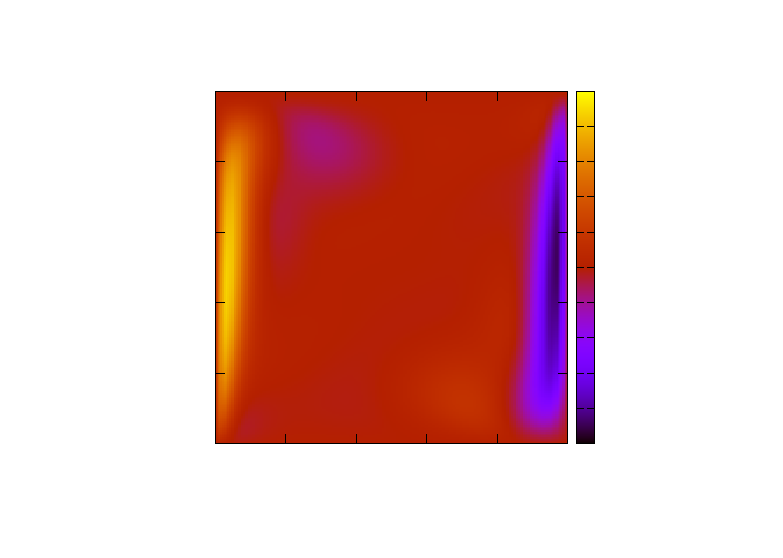
\includegraphics{Buoyancy/v6}}%
    \gplfronttext
  \end{picture}%
\endgroup
}
		\caption{$Ra=10^{6}$}
		\label{vplotRa6}
	\end{subfigure}
	\caption{Contour plots of the vertical velocity}
	\label{vplotDiffHeated}
\end{figure}

Figure \ref{uplotDiffHeated} displays the horizontal velocity in the cavity for the studied Rayleigh numbers. In the case of the horizontal velocity, it can be seen that the hot fluid (in top) moves to the colder zone as expected, displacing the cold fluid (at the bottom) to the left. At low Rayleigh numbers, the maximum velocities, positive and negative, are in the top and bottom middle of the cavity; but at higher Ra, the maximum velocities move to the right and left corners respectively.

For the vertical velocity (figures \ref{vplotDiffHeated}), the hot fluid (left) moves upwards, whereas the cold fluid (right), that has a higher density, moves downwards. However, the centre of the cavity does not move. When the Rayleigh number increases, the areas with important vertical velocities are stretched, increasing the velocity gradient in the walls. It is also important to notice that in figures \ref{vplotRa5} and \ref{vplotRa6} there is a some downwards movement in the left half of the cavity. This suggests that the fluid movement becomes more complex at higher Ra.

As a conclusion, regarding the horizontal and vertical velocities, it can be said the the fluid moves in a clock-wise direction, but as the Rayleigh number increases, its rotation becomes more complex.

Finally, it is important to verify the results. Table \ref{ComparisonDiffHeated} displays a comparison between the results and the reference values, and table \ref{ErrorDiffHeated} the error. The parameters studied are listed below:
\begin{itemize}
	\item $u_{max}$: Maximum horizontal velocity on the vertical mid-plane of the cavity and its location.
	\item $v_{max}$: Maximum vertical velocity on the horizontal mid-plane of the cavity and its location.
	\item $\overbar{Nu}$: Average Nusselt number throughout the cavity.
	\item $Nu_{1/2}$: Average Nusselt number on the vertical mid-plane of the cavity.
	\item $Nu_{0}$: Average Nusselt number on the vertical boundary of the cavity at $x=0$.
	\item $Nu_{max}$: Maximum value of the local Nusselt number on the left wall $x=0$ and its location.
	\item $Nu_{min}$: Minimum value of the local Nusselt number on the left wall $x=0$ and its location.
\end{itemize}
\begin{table}[h]
	\centering
	\begin{tabular}{c|c|c|c|c|c|c|c|c|}
		\cline{2-9}
		\multicolumn{1}{l|}{}       & \multicolumn{2}{c|}{$Ra=10^{3}$} & \multicolumn{2}{c|}{$Ra=10^{4}$} & \multicolumn{2}{c|}{$Ra=10^{5}$} & \multicolumn{2}{c|}{$Ra=10^{6}$} \\ \cline{2-9} 
		\multicolumn{1}{l|}{}       & Calculated                & Bench                & Calculated                & Bench                & Calculated                & Bench                & Calculated                & Bench                \\ \hline
		\multicolumn{1}{|c|}{$u_{max}$}  & 3.70837                   & 3.649                & 16.1984                   & 16.178               & 34.5076                   & 34.73                & 66.1923                   & 64.63                \\ \hline
		\multicolumn{1}{|c|}{$y$}     & 0.81                      & 0.813                & 0.83                      & 0.823                & 0.85                      & 0.855                & 0.85                      & 0.85                 \\ \hline
		\multicolumn{1}{|c|}{$v_{max}$}  & 3.9083                    & 3.697                & 19.6482                   & 19.617               & 68.663                    & 68.59                & 220.23                    & 219.36               \\ \hline
		\multicolumn{1}{|c|}{$x$}     & 0.17                      & 0.178                & 0.11                      & 0.119                & 0.07                      & 0.066                & 0.03                      & 0.0379               \\ \hline
		\multicolumn{1}{|c|}{$\overbar{Nu}$} & 1.122                     & 1.118                & 2.24403                   & 2.243                & 4.53504                   & 4.519                & 9.03057                   & 8.8                  \\ \hline
		\multicolumn{1}{|c|}{$Nu_{1/2}$}  & 1.09509                   & 1.118                & 2.22832                   & 2.243                & 4.53594                   & 4.519                & 9.11047                   & 8.799                \\ \hline
		\multicolumn{1}{|c|}{$Nu_{0}$}   & 1.36657                   & 1.117                & 2.33106                   & 2.238                & 4.66892                   & 4.509                & 9.41921                   & 8.817                \\ \hline
		\multicolumn{1}{|c|}{$Nu_{max}$} & 1.7952                    & 1.505                & 3.62633                   & 3.528                & 8.04508                   & 7.717                & 20.0189                   & 17.925               \\ \hline
		\multicolumn{1}{|c|}{$y$}     & 0.09                      & 0.092                & 0.15                      & 0.143                & 0.07                      & 0.081                & 0.03                      & 0.0378               \\ \hline
		\multicolumn{1}{|c|}{$Nu_{min}$} & 0.872725                  & 0.692                & 0.616051                  & 0.586                & 0.763572                  & 0.729                & 1.06205                   & 0.989                \\ \hline
		\multicolumn{1}{|c|}{$y$}     & 1                         & 1                    & 1                         & 1                    & 1                         & 1                    & 1                         & 1                    \\ \hline
	\end{tabular}
\caption[Comparison between the benchmark solution and the calculated one]{Comparison between the benchmark solution and the calculated one \cite{DeVahlDavis1983}}
\label{ComparisonDiffHeated}
\end{table}

In some cases the error can be bigger than 5\%, especially in the Nusselt numbers on the left wall and in the locations of the values. In the case of the coordinates, the error may be due to the mesh used. In the calculations the mesh was coarser than the one used in the reference solution. All in all, the results that have higher error are the ones of the lowest and highest Rayleigh numbers.

\begin{table}[h]
	\centering
	\begin{tabular}{c|c|c|c|c|}
		\cline{2-5}
		\multicolumn{1}{l|}{}       & $Ra=10^{3}$ & $Ra=10^{4}$ & $Ra=10^{5}$ & $Ra=10^{6}$ \\ \hline
		\multicolumn{1}{|c|}{$u_{max}$}  & -1.627\%                    & -0.126\%                    & 0.640\%                     & -2.417\%                    \\ \hline
		\multicolumn{1}{|c|}{$y$}     & 0.369\%                     & -0.851\%                    & 0.585\%                     & 0.000\%                     \\ \hline
		\multicolumn{1}{|c|}{$v_{max}$}  & -5.715\%                    & -0.159\%                    & -0.106\%                    & -0.397\%                    \\ \hline
		\multicolumn{1}{|c|}{$x$}     & 4.494\%                     & 7.563\%                     & -6.061\%                    & 20.844\%                    \\ \hline
		\multicolumn{1}{|c|}{$\overbar{Nu}$} & -0.358\%                    & -0.046\%                    & -0.355\%                    & -2.620\%                    \\ \hline
		\multicolumn{1}{|c|}{$Nu_{1/2}$}  & 2.049\%                     & 0.654\%                     & -0.375\%                    & -3.540\%                    \\ \hline
		\multicolumn{1}{|c|}{$Nu_{0}$}   & -22.343\%                   & -4.158\%                    & -3.547\%                    & -6.830\%                    \\ \hline
		\multicolumn{1}{|c|}{$Nu_{max}$} & -19.282\%                   & -2.787\%                    & -4.251\%                    & -11.681\%                   \\ \hline
		\multicolumn{1}{|c|}{$y$}     & 2.174\%                     & -4.895\%                    & 13.580\%                    & 20.635\%                    \\ \hline
		\multicolumn{1}{|c|}{$Nu_{min}$} & -26.116\%                   & -5.128\%                    & -4.742\%                    & -7.386\%                    \\ \hline
		\multicolumn{1}{|c|}{$y$}     & 0.000\%                     & 0.000\%                     & 0.000\%                     & 0.000\%                     \\ \hline
	\end{tabular}
	\caption{Percentage of error between the benchmark solution and the calculated one}
	\label{ErrorDiffHeated}
\end{table}